\input{../../tex_header}

\title{Chapter 22 Solusion}
\date{12/1/2021}

\begin{document}
\maketitle

\section*{22.1}

\subsection*{22.1-1}

out-degree: $\Theta(V + E)$ by simply counting the size of each adjacency list.

\begin{minted}[xleftmargin=20pt,linenos]{cpp}
std::vector<int> OutDegree(const Graph& graph)
{
    size_t v_size, i;
    v_size = graph.adj.size();
    std::vector<int> degree(v_size);
    for (i = 0; i < v_size; ++i)
    {
        // assume graph.adj[i].size() takes O(n) 
        // where n is size of  graph.adj[i]
        degree[i] = graph.adj[i].size();
    }
    return degree;
}
\end{minted}

in-degree: $\Theta(V + E)$ by maintaining a counting table: 
each entry of the table is the counter for in-degree of the specific vertex.

\begin{minted}[xleftmargin=20pt,linenos]{cpp}
std::vector<int> InDegree(const Graph& graph)
{
    size_t v_size, i;
    v_size = graph.adj.size();
    std::vector<int> degree(v_size);
    for (i = 0; i < v_size; ++i)
    {
        for (int v : graph.adj[i])
        {
            ++degree[v];
        }
    }
    return degree;
}
\end{minted}

\subsection*{22.1-2}

Consider the following binary tree:

\Tree [.7 
[.5
    [.1 ] [.2 ]
] [.6
    [.3 ] [.4 ]
]
]

We have the following adjacency-list representation:

\begin{tikzpicture}[>=stealth] 

\matrix (M) [matrix of nodes,
   column sep=-\pgflinewidth,
   row sep=0mm,
   nodes in empty cells,
   nodes={draw, fill=gray!20,
     minimum width=.5cm, outer sep=0pt,
     minimum height=.7cm, anchor=center}, 
   column 1/.style={nodes={minimum height=.8cm}}]
{ 
  &[2mm] 5 & /  \\ 
  &[2mm] 5 & /  \\ 
  &[2mm] 6 & /  \\ 
  &[2mm] 6 & /  \\ 
  & 1 & &[2mm] 2 & &[2mm] 7 & / \\ 
  & 3 & & 4 & & 7 & / \\ 
  & 5 & & 6 & / \\
}; 

\foreach \i in {1,2,3,4,5,6,7}{ 
 \path (M-\i-1) [late options={label=left:\i}]; 
 \draw[->] (M-\i-1)--(M-\i-2.west); 
} 

\draw[->] (M-5-3.center)--(M-5-4.west); 
\draw[->] (M-5-5.center)--(M-5-6.west); 
\draw[->] (M-6-3.center)--(M-6-4.west); 
\draw[->] (M-6-5.center)--(M-6-6.west); 
\draw[->] (M-7-3.center)--(M-7-4.west); 

\end{tikzpicture}

We have the following adjacency-matrix representation:

\begin{tabular}{c c c c c c c c}
    ~ & 1 & 2 & 3 & 4 & 5 & 6 & 7 \\ \cline{2-8}
    \multicolumn{1}{c|}{1} & 0 & 0 & 0 & 0 & 1 & 0 & \multicolumn{1}{c|}{0} \\
    \multicolumn{1}{c|}{2} & 0 & 0 & 0 & 0 & 1 & 0 & \multicolumn{1}{c|}{0} \\
    \multicolumn{1}{c|}{3} & 0 & 0 & 0 & 0 & 0 & 1 & \multicolumn{1}{c|}{0} \\
    \multicolumn{1}{c|}{4} & 0 & 0 & 0 & 0 & 0 & 1 & \multicolumn{1}{c|}{0} \\
    \multicolumn{1}{c|}{5} & 1 & 1 & 0 & 0 & 0 & 0 & \multicolumn{1}{c|}{1} \\
    \multicolumn{1}{c|}{6} & 0 & 0 & 1 & 1 & 0 & 0 & \multicolumn{1}{c|}{1} \\
    \multicolumn{1}{c|}{7} & 0 & 0 & 0 & 0 & 1 & 1 & \multicolumn{1}{c|}{0} \\ \cline{2-8}
\end{tabular}

\subsection*{22.1-3}

We can compute $G^T$ from $G$ 
for the adjacency-list representation in $\Theta(V + E)$
by the following algorithm:

\begin{minted}[xleftmargin=20pt,linenos]{cpp}
AdjListGraph Transpose(const AdjListGraph& graph)
{
    size_t size, u;
    size = graph.adj.size();
    AdjListGraph target(size);
    for (u = 0; u < size; ++u)
    {
        for (int v : graph.adj[u])
        {
            target.adj[v].push_back(u);
        }
    }
    return target;
}
\end{minted}

We can compute $G^T$ from $G$ 
for the adjacency-matrix representation in $\Theta(V^2)$
by the following algorithm:
    
\begin{minted}[xleftmargin=20pt,linenos]{cpp}
AdjMatrixGraph Transpose(const AdjMatrixGraph& graph)
{
    size_t size, u, v;
    size = graph.adj.size();
    AdjMatrixGraph target(size);
    for (u = 0; u < size; ++u)
    {
        for (v = 0; v < size; ++v)
        {
            target.adj[v][u] = graph.adj[u][v];
        }
    }
    return target;
}
\end{minted}

\subsection*{22.1-4}

\begin{minted}[xleftmargin=20pt,linenos]{cpp}
AdjListGraph Equivalent(const AdjListGraph& graph)
{
    size_t size, u;
    size = graph.adj.size();
    AdjListGraph target(size);
    std::vector<bool> edge_usage;
    for (u = 0; u < size; ++u)
    {
        edge_usage = std::vector<bool>(size, false);
        edge_usage[u] = true;
        for (int v : graph.adj[u])
        {
            if (edge_usage[v] == false)
            {
                target.adj[u].push_back(v);
                edge_usage[v] = true;
            }
        }
    }
    return target;
}
\end{minted}

\subsection*{22.1-5}

We can compute $G^2$ from $G$ 
for the adjacency-list representation in $O(VE)$
by the following algorithm:

\begin{minted}[xleftmargin=20pt,linenos]{cpp}
AdjListGraph Square(const AdjListGraph& graph)
{
    size_t size, u;
    size = graph.adj.size();
    AdjListGraph result(size);
    for (u = 0; u < size; ++u)
    {
        for (int v : graph.adj[u])
        {
            result.adj[u].push_back(v);
            for (int w : graph.adj[v])
            {
                result.adj[u].push_back(w);
            }
        }
    }
    return result;
}
\end{minted}

We can compute $G^2$ from $G$ 
for the adjacency-matrix representation in $\Theta(V^3)$
by the following algorithm
(note that $G^2$ might be a not simple graph):
    
\begin{minted}[xleftmargin=20pt,linenos]{cpp}
AdjMatrixGraph Square(const AdjMatrixGraph& graph)
{
    size_t size, u, v, w;
    size = graph.Rows();
    AdjMatrixGraph result(size, size);
    for (u = 0; u < size; ++u)
    {
        for (v = 0; v < size; ++v)
        {
            if (graph[u][v])
            {
                result[u][v] = true;
                for (w = 0; w < size; ++w)
                {
                    if (graph[v][w])
                    {
                        result[u][w] = true;
                    }
                }
            }
        }
    }
    return result;
}
\end{minted}

We also can optimate computation of $G^2$ from $G$
by using Strassen algorithm.

\begin{lemma}
    Let $A=(a_{ij})$ be a $n \times n$ nonnegative matrix and $B=A^2=(b_{ij})$.
    Then $b_{uw} > 0$ if and only if 
    there exists some integer $v \in [1,n]$ such that $a_{uv} > 0$ and $a_{vw} > 0$.
\end{lemma}

\begin{proof}
    Contrapositive: 
    $b_{uw} = 0$ 
    $\Longleftrightarrow$
    $(\forall v \in \ZZ_{[1,n]}, a_{uv} = 0 \vee a_{vw} = 0)$

    According to equation (4.8) on page 75, we have

    \begin{equation*}
        b_{uw} = \sum\limits_{v=1}^{n} a_{uv} \cdot a_{vw}.
    \end{equation*}

    Note $A$ is nonnegative matrix.
    Clearly, $b_{uw} = 0$ if and only if
    $a_{uv}=0$ or $a_{vw}=0$ for all integer $v \in [1,n]$
\end{proof}

\begin{claim}
    Let $A=(a_{ij})$ be the adjacency-matrix repressentations of graph $G=(V,E)$.
    Let $B = A^2=(b_{ij})$.
    Then $b_{uw} > 0$ if and only if 
    there exists a path with exactly two edges between $u$ and $w$.
\end{claim}

\begin{proof}
    To prove the claim, we just need to show that 
    ``there exists a path with exactly two edges between $u$ and $w$''
    is equivalent to
    ``there exists some integer $v \in [1,n]$ such that $a_{uv} > 0$ and $a_{vw} > 0$''
    so we can utilize lemma 1.
    Let $v \in V$.
    We have $(u,v) \in E$ if and only if $a_{uv} > 0$.
    Similarly, $(v,w) \in E$ if and only if $a_{vw} > 0$.
    Also, $(u,v) \in E$ and $(v,w) \in E$ means
    there exists a path: $u \rightarrow v \rightarrow w$.
\end{proof}

Therefore, we have the following algorithm run in $\Theta(|V|^{\lg 7})$:

\begin{minted}[xleftmargin=20pt,linenos]{cpp}
AdjMatrixGraph SquareByStrassen(const AdjMatrixGraph& graph)
{
    size_t size, u, v, w;
    size = graph.Rows();
    AdjMatrixGraph result = StrassenMultiplication(graph, graph);
    for (u = 0; u < size; ++u)
    {
        for (v = 0; v < size; ++v)
        {
            if (graph[u][v])
            {
                result[u][v] = 1;
            }
        }
    }
    return result;
}
\end{minted}

\subsection*{22.1-6}

Notice that we can check whether a vertex is a universal sink in $\Theta(|V|)$.
However, it will take $O(|V|^2)$ to check all vertex precisely.
So, we want to constraint to a unique possible vertex and check that unique possible vertex.

\begin{claim}
    $v \in V$ is a universal sink if and only if
    $(\forall w \in V, a_{vw} = 0)$
    and 
    $(\forall u \in V \setminus \{ v \}, a_{uv} = 1)$. 
\end{claim}

Then we have

\begin{equation*}
    \begin{cases}
        a_{uv} = 1 & \text{ implies $u$ is not a universal sink,} \\
        a_{uv} = 0 \wedge u \neq v & \text{ implies $v$ is not a universal sink.}
    \end{cases}
\end{equation*}

Thus we can eliminate a candidate vertex either $u$ or $v$ in $\Theta(1)$ 
by access $a_{uv}$ if $u \neq v$.

Therefore, we have the following algorithm run in $\Theta(|V|)$:

\begin{minted}[xleftmargin=20pt,linenos]{cpp}
// graph must be a square matrix
// return vertex of universal sink
// return -1 if universal sink not exist
int UniversalSink(const Matrix& graph)
{
    size_t size, u, v;
    size = graph.size();
    // eliminate candidates
    u = 0;
    v = 1;
    while (v < size)
    {
        if (graph[u][v])
        {
            ++u;
            if (u == v)
            {
                ++v;
            }
        }
        else
        {
            ++v;
        }
    }
    // test the possible vertex u by claim 3
    for (v = 0; v < size; ++v)
    {
        if (graph[u][v])
            return -1;
    }
    for (v = 0; v < size; ++v)
    {
        if (graph[v][u] == false && u != v)
            return -1;
    }
    return u;
}
\end{minted}

The following algorithm runs in $\Theta(|V|)$ also:

\begin{minted}[xleftmargin=20pt,linenos]{cpp}
int UniversalSinkAnother(const Matrix& graph)
{
    size_t size, u, v;
    size = graph.size();
    u = 0;
    v = 0;
    while (u < size && v < size)
    {
        if (graph[u][v])
        {
            ++u;
        }
        else
        {
            ++v;
        }
    }
    if (u >= size)
        return -1;
    for (v = 0; v < size; ++v)
    {
        if (graph[u][v])
            return -1;
    }
    for (v = 0; v < size; ++v)
    {
        if (graph[v][u] == false && u != v)
            return -1;
    }
    return u;
}
\end{minted}

\subsection*{22.1-7}

Let matrix $C = B^T = (c_{ij})$.
This says $C$ is a $|E| \times |V|$ matrix,
and $c_{ij} = b_{ji}$.
Let $D = BB^T = (d_{ij})$.
Hence we have

\begin{equation*}
    d_{ij} = \sum\limits_{k \in E} b_{ik} c_{kj} = \sum\limits_{k \in E} b_{ik} b_{jk}
\end{equation*}

In conclusion, the meaning of $d_{ij}$ depends on whether $i=j$.

\textbf{Case 1}
$i = j$

$b_{ik}b_{jk} = b_{ik} = 1 = 1 \cdot 1 = -1 \cdot -1$ implies edge $k$ enters or leaves vertex $i$. 

$b_{ik}b_{jk} = b_{ik} = 0$ implies edge $k$ does not connect to vertex $i$. 

$b_{ik}b_{jk} = b_{ik} = -1$ is impossible since $b_{ik} = b_{jk}$.

Hence $d_{ij}$ means the total degree (in-degree + out-degree) of vertex $i$.

\textbf{Case 2}
$i \neq j$

$b_{ik}b_{jk} = 1 = 1 \cdot 1 = -1 \cdot -1$ is impossible 
since edge $k$ cannot enter $i$ and $j$ simultaneously,
and edge $k$ cannot leave $i$ and $j$ simultaneously.

$b_{ik}b_{jk} = 0$ implies edge $k$ does not connect to vertex $i$ and $j$. 

$b_{ik}b_{jk} = -1$ implies edge $k$ leaves vertex $i$ and enters $j$,
or edge $k$ leaves vertex $j$ and enters $i$. 

Hence $-d_{ij}$ means the number of edges connect to vertex $i$ and $j$ simultaneously.

\subsection*{22.1-8}

Expected time to determine whether an edge is in the graph: $\Theta(1)$.

Disadvantage to use hash table: 
1. we are not able to handle graphs that are not simple;
2. the worst case take $\Theta(|V|)$ time.

Suggest: 
utilize red-black trees containing keys $v$ much that $(u,v) \in E$;
add a counter (counter for unweighted graph; list for weighted graph) 
to the attributes of each node in the red-black tree to handle graphs that are not simple.

Disadvantage compared to the hash table:
expect time of red-black tree is $\Theta(\lg n)$
where $n$ is the size of elements in the red-black tree. 

\section*{22.2}

\subsection*{22.2-1}

vertex 1: $d = \infty$, $\pi = NIL$.

vertex 2: $d = 3$, $\pi = 4$.

vertex 3: $d = 0$, $\pi = NIL$.

vertex 4: $d = 2$, $\pi = 5$.

vertex 5: $d = 1$, $\pi = 3$.

vertex 6: $d = 1$, $\pi = 3$.

\subsection*{22.2-2}

vertex r: $d = 4$, $\pi = s$.

vertex s: $d = 3$, $\pi = w$.

vertex t: $d = 1$, $\pi = u$.

vertex u: $d = 0$, $\pi = NIL$.

vertex v: $d = 5$, $\pi = r$.

vertex w: $d = 2$, $\pi = x$.

vertex x: $d = 1$, $\pi = u$.

vertex y: $d = 1$, $\pi = u$.

\subsection*{22.2-3}

We can replace all "GRAY"s with "BLACK"s.
Notice line 13 is the only place to check color,
and it only checks whether or not the vertex is "WHITE".
Hence, as long as we can make sure all non-white vertex are in non-"WHITE" color,
our algorithm works.

\begin{minted}[xleftmargin=20pt,linenos]{cpp}
std::list<int> BFS(Graph& graph, int src_idx)
{
    int u_idx, v_idx;
    std::list<int> discover_result;
    std::queue<int> q;
    for (Vertex& u : graph.vertices)
    {
        u.color = Color::kWhite;
        u.distance = INT_MAX;
        u.prev = -1;
    }
    graph.vertices[src_idx].color = Color::kNonWhite;
    graph.vertices[src_idx].distance = 0;
    graph.vertices[src_idx].prev = -1;
    q.push(src_idx);
    while (q.empty() == false)
    {
        u_idx = q.front();
        q.pop();
        discover_result.push_back(u_idx);
        Vertex& u = graph.vertices[u_idx];
        for (int v_idx : graph.adj[u_idx])
        {
            Vertex& v = graph.vertices[v_idx];
            if (v.color == Color::kWhite)
            {
                v.color = Color::kNonWhite;
                v.distance = u.distance + 1;
                v.prev = u_idx;
                q.push(v_idx);
            }
        }
    }
    return discover_result;
}
\end{minted}

\subsection*{22.2-4}

$O(V^2)$ since we need to iterate all entries in the matrix.

\begin{minted}[xleftmargin=20pt,linenos]{cpp}
std::list<int> BFS(Graph& graph, int src_idx)
{
    int u_idx, v_idx;
    std::list<int> discover_result;
    std::queue<int> q;
    for (Vertex& u : graph.vertices)
    {
        u.color = Color::kWhite;
        u.distance = INT_MAX;
        u.prev = -1;
    }
    graph.vertices[src_idx].color = Color::kGray;
    graph.vertices[src_idx].distance = 0;
    graph.vertices[src_idx].prev = -1;
    q.push(src_idx);
    while (q.empty() == false)
    {
        u_idx = q.front();
        q.pop();
        discover_result.push_back(u_idx);
        Vertex& u = graph.vertices[u_idx];
        for (v_idx = 0; v_idx < graph.size; ++v_idx)
        {
            if (graph.adj[u_idx][v_idx])
            {
                Vertex& v = graph.vertices[v_idx];
                if (v.color == Color::kWhite)
                {
                    v.color = Color::kGray;
                    v.distance = u.distance + 1;
                    v.prev = u_idx;
                    q.push(v_idx);
                }
            }
        }
        u.color = Color::kBlack;
    }
    return discover_result;
}
\end{minted}

\subsection*{22.2-5}

For all reachable vertices $v \in V$,
we have $v.d = \delta(s,v)$ by Theorem 22.5.
For unreachable vertices $v \in V$,
we have $v.d = \infty = \delta(s,v)$.
Since $\delta(s,v)$ is independent of the order in which
the vertices appear in each adjacency list,
so does $v.d$ for all $v \in V$.

If $t$ is in front of $x$ in the adjacency list of $w$,
then $t$ will be enqueued before $x$ enqueue,
and $u.\pi = t$, so $(t,u) \in E_\pi$.
If $t$ is in after $x$ in the adjacency list of $w$,
then $t$ will be enqueued after $x$ enqueue,
and $u.\pi = x$, so $(x,u) \in E_\pi$.

\subsection*{22.2-6}

Consider the following directed graph $G = (V,E)$:

\begin{tikzpicture}
    \tikzset{vertex/.style = {shape=circle,draw,minimum size=2em}}
    \tikzset{edge/.style = {->,> = latex'}}
    % vertices
    \node[vertex] (a) at  (0,0) {$a$};
    \node[vertex] (s) at  (2,2) {$s$};
    \node[vertex] (b) at  (4,0) {$b$};
    \node[vertex] (c) at  (0,-4) {$c$};
    \node[vertex] (d) at  (4,-4) {$d$};
    %edges
    \draw[edge] (s) to (a);
    \draw[edge] (s) to (b);
    \draw[edge] (a) to (c);
    \draw[edge] (a) to (d);
    \draw[edge] (b) to (c);
    \draw[edge] (b) to (d);
\end{tikzpicture}

Consider $E_\pi = \{ (s,a), (s,b), (a,c), (b,d) \}$.
This $E_\pi$ cannot be produced by running BFS on $G$.

The only two possible predecessor subgraph is

\begin{equation*}
    (V, \{ (s,a), (s,b), (a,c), (a,d) \})
\end{equation*}

and

\begin{equation*}
    (V, \{ (s,b), (s,a), (b,c), (b,d) \}).
\end{equation*}

\subsection*{22.2-7}

Let $G=(V,E)$ be an undirected graph.

Let each vertex $v \in V$ represent a professional wrestler,
and let each edge $e \in E$ represent a rivalry.

\begin{minted}[xleftmargin=20pt,linenos]{cpp}
bool DesignateWrestlerType(Graph& graph)
{
    int u_idx, v_idx;
    std::queue<int> q;
    for (Vertex& u : graph.vertices)
    {
        u.color = Color::kWhite;
    }
    graph.vertices[0].color = Color::kNonWhite;
    graph.vertices[0].type = WrestlerType::kBabyfaces;
    q.push(0);
    while (q.empty() == false)
    {
        u_idx = q.front();
        q.pop();
        Vertex& u = graph.vertices[u_idx];
        for (int v_idx : graph.adj[u_idx])
        {
            Vertex& v = graph.vertices[v_idx];
            if (v.color == Color::kWhite)
            {
                v.color = Color::kNonWhite;
                graph.vertices[v_idx].type = (u.type == WrestlerType::kBabyfaces) ? 
                    WrestlerType::kHeels : WrestlerType::kBabyfaces;
                q.push(v_idx);
            }
            else
            {
                if (u.type == v.type)
                    return false;
            }
        }
    }
    return true;
}
\end{minted}

\subsection*{22.2-8}

According to Theorem B.2 (Properties of free trees),
We have $T$ is connected, acyclic, and $|E| = |V| - 1$.
This says we can do BFS in $O(|V| + |E|) = O(|V| + |V| - 1) = O(|V|)$ time.
If we can do constant times BFS, we will be able to find diameter in $O(|V|)$ time.

Let arbitrary node $s \in V$ be the sourse node of BFS.
Since $T$ is connected, all nodes in $V$ are reachable.
After performing BFS on $T$ from the souece node $s$,
we have $v.d = \delta(s,v)$ for each $v \in V$.
Let $s$ be the root node of the tree $T$.
Then $v.d$ is the depth of node $v$ is the tree
since any two vertices in a tree are connected by a unique simple path (Theorem B.2 (2))
and the length of the path from $s$ to $v$ is $\delta(s,v)$, which is depth of node $v$.
We can recursive traverse the tree to get the height of each node based on depth,
and we can get the longest path containes the root of the subtree by height of children of the root.

Since BFS takes $O(|V|)$ and traverses tree takes $O(|V|)$,
our algorithm run in $O(|V|)$.

\begin{minted}[xleftmargin=20pt,linenos]{cpp}
int DiameterAux(Graph& graph, int subtree_root_idx)
{
    int first_largest_h, second_largest_h, longest_path_length;
    first_largest_h = -1;
    second_largest_h = -1;
    longest_path_length = INT_MIN;
    Vertex& subtree_root = graph.vertices[subtree_root_idx];
    for (int child_idx : graph.adj[subtree_root_idx])
    {
        if (child_idx != subtree_root.prev)
        {
            Vertex& child = graph.vertices[child_idx];
            longest_path_length = std::max(longest_path_length, 
                DiameterAux(graph, child_idx));
            if (child.height > first_largest_h)
            {
                second_largest_h = first_largest_h;
                first_largest_h = child.height;
            }
            else if (child.height > second_largest_h)
            {
                second_largest_h = child.height;
            }
        }
    }
    subtree_root.height = first_largest_h + 1;
    longest_path_length = std::max(longest_path_length, 
                first_largest_h + second_largest_h + 2);
    return longest_path_length;
}

int Diameter(Graph& graph)
{
    int u_idx, v_idx;
    std::queue<int> q;
    // let vertex 0 be the root node
    graph.vertices[0].depth = 0;
    graph.vertices[0].prev = -1;
    q.push(0);
    while (q.empty() == false)
    {
        u_idx = q.front();
        q.pop();
        Vertex& u = graph.vertices[u_idx];
        for (int v_idx : graph.adj[u_idx])
        {
            if (v_idx != u.prev)
            {
                Vertex& v = graph.vertices[v_idx];
                v.depth = u.depth + 1;
                v.prev = u_idx;
                q.push(v_idx);
            }
        }
    }
    return DiameterAux(graph, 0);
}
\end{minted}

\subsection*{22.2-9}

\begin{minted}[xleftmargin=20pt,linenos]{cpp}
std::list< std::pair<int, int> > TraverseEdge(Graph& graph, int src_idx)
{
    int u_idx, v_idx;
    std::list< std::pair<int, int> > traverse_result;
    std::list< std::pair<int, int> >::iterator result_it;
    std::queue<int> q;
    for (Vertex& u : graph.vertices)
    {
        u.color = Color::kWhite;
    }
    graph.vertices[src_idx].color = Color::kGray;
    graph.vertices[src_idx].result_pos = traverse_result.end();
    q.push(src_idx);
    while (q.empty() == false)
    {
        u_idx = q.front();
        q.pop();
        Vertex& u = graph.vertices[u_idx];
        result_it = u.result_pos;
        for (int v_idx : graph.adj[u_idx])
        {
            Vertex& v = graph.vertices[v_idx];
            if (v.color == Color::kWhite)
            {
                v.color = Color::kGray;
                traverse_result.emplace(result_it, u_idx, v_idx);
                v.result_pos = 
                    traverse_result.emplace(result_it, v_idx, u_idx);
                q.push(v_idx);
            }
            else if (v.color == Color::kGray)
            {
                traverse_result.emplace(result_it, u_idx, v_idx);
                traverse_result.emplace(result_it, v_idx, u_idx);
            }
        }
        u.color = Color::kBlack;
    }
    return traverse_result;
}
\end{minted}

Let each spot of the maze be a vertex in $V$.
If there is no wall between two spots, 
we add an edge to connect two vertices.
Then we traverse each edge in $E$ by using the above algorithm
to find the way out of the maze.

\section*{22.3}

\subsection*{22.3-1}

Directed:

\begin{tabular}{l|c c c}
    \diagbox{i}{j} & WHITE & GRAY & BLACK \\
    \hline
    W   & tree/back/forward/cross & back/cross & cross \\
    G   & tree/forward & tree/back/forward & tree/forward/cross \\
    B   & N/A & back & tree/back/forward/cross
\end{tabular}

Undirected:

\begin{tabular}{l|c c c}
    \diagbox{i}{j} & WHITE & GRAY & BLACK \\
    \hline
    W   & tree/back & tree/back & N/A \\
    G   & tree/back & tree/back & tree/back \\
    B   & N/A & tree/back & tree/back
\end{tabular}

\subsection*{22.3-2}

\noindent
Discovery and finish time:

\begin{description}
    \item[q] 1/16
    \item[s] 2/7
    \item[v] 3/6
    \item[w] 4/5
    \item[t] 8/15
    \item[x] 9/12
    \item[z] 10/11
    \item[y] 13/14
    \item[r] 17/20
    \item[u] 18/19
\end{description}

\noindent
Classification of each edge:

\begin{description}
    \item[(q,s)] tree
    \item[(s,v)] tree
    \item[(v,w)] tree
    \item[(w,s)] back
    \item[(q,t)] tree
    \item[(t,x)] tree
    \item[(x,z)] tree
    \item[(z,x)] back
    \item[(t,y)] tree
    \item[(y,q)] back
    \item[(q,w)] forward
    \item[(r,u)] tree
    \item[(u,y)] cross
    \item[(r,y)] cross
\end{description}

\subsection*{22.3-3}

(u (v (y (x x) y) v) u) (w (z z) w)

\subsection*{22.3-4}

The algorithm only check if the color is white or non white, 
so we can use only two colors.

\begin{minted}[xleftmargin=20pt,linenos]{cpp}
void DFSVisit(Graph& graph, int u_idx, int& time)
{
    Vertex& u = graph.vertices[u_idx];
    ++time;
    u.discovery_time = time;
    u.color = Color::kNonWhite;
    for (int v_idx : graph.adj[u_idx])
    {
        Vertex& v = graph.vertices[v_idx];
        if (v.color == Color::kWhite)
        {
            v.prev = u_idx;
            DFSVisit(graph, v_idx, time);
        }
    }
    ++time;
    u.finishing_time = time;
}

void DFS(Graph& graph)
{
    int time, u_idx;
    for (Vertex& u : graph.vertices)
    {
        u.color = Color::kWhite;
    }
    time = 0;
    for (u_idx = 0; u_idx < graph.size; ++u_idx)
    {
        Vertex& u = graph.vertices[u_idx];
        if (u.color == Color::kWhite)
        {
            u.prev = -1;
            DFSVisit(graph, u_idx, time);
        }
    }
}
\end{minted}

\subsection*{22.3-5}

\subsubsection*{(a)}

\begin{proof}
    Edge $(u,v)$ is a tree edge or forward edge if and only if
    $v$ is a proper descendant of $u$.
    By Corollary 22.8 (Nesting of descendants' intervals),
    we have $u.d < v.d < v.f < u.f$ if and only if
    $v$ is a proper descendant of $u$.
\end{proof}

\subsubsection*{(b)}

\begin{proof}
    Edge $(u,v)$ is a back edge if and only if
    $u$ is a descendant of $v$ (include self-loop).
    By Theorem 22.7 (Parenthesis theorem),
    we have $v.d\leq< u.d < u.f \leq v.f$ if and only if
    $u$ is a descendant of $v$ immediately.
\end{proof}

\subsubsection*{(c)}

\begin{proof}
    Edge $(u,v)$ is a cross edge if and only if
    $u$ is neither descendant of $v$ nor ancestor of $v$.
    By Theorem 22.7 (Parenthesis theorem),
    we have $v.d < v.f < u.d < u.f$ or $u.d < u.f < v.d < v.f$ if and only if
    $u$ is neither descendant of $v$ nor ancestor of $v$.
    Thus, we have $v.d < v.f < u.d < u.f$ $\Longrightarrow$ $(u,v)$ is a cross edge.
    
    We claim $(u,v)$ is a cross edge $\Longrightarrow$ $v.d < v.f < u.d < u.f$.
    Assume $u.d < u.f < v.d < v.f$, for the purpose of contradiction.
    This says $u$ is black and $v$ is white at some point during the DFS.
    However, there is a edge from $u$ to $v$, which is a contradiction.
\end{proof}

\subsection*{22.3-6}

\begin{proof}
    By definition of tree edge, edge $(u,v)$ is classified as a tree edge 
    if $v$ is first discovered by exploring edge $(u,v)$,
    which is equivalent to $(u,v)$ is encountered first.
    By Theorem 22.10, 
    every edge in an undirected graph is either a tree edge or a back edge.
    Thus, if $(u,v)$ is not classified as a tree edge,
    $(u,v)$ is classified as a back edge, 
    which is equivalent to $(v,u)$ is encountered first.
\end{proof}

\subsection*{22.3-7}

\begin{minted}[xleftmargin=20pt,linenos]{cpp}
struct StackElement
{
    int vertex_idx;
    AdjList::iterator adj_it_curr;
    AdjList::iterator adj_it_end;
};

void DFS(Graph& graph)
{
    int time, u_idx, v_idx;
    std::stack< StackElement > path;
    AdjList vertices_list;
    for (u_idx = 0; u_idx < graph.size; ++u_idx)
    {
        Vertex& u = graph.vertices[u_idx];
        u.color = Color::kWhite;
        vertices_list.push_back(u_idx);
    }
    time = 0;
    path.push({ -1, vertices_list.begin(), vertices_list.end() });
    while (true)
    {
        u_idx = path.top().vertex_idx;
        AdjList::iterator& v_it = path.top().adj_it_curr;
        if (v_it == path.top().adj_it_end)
        {
            path.pop();
            if (path.empty())
                break;
            Vertex& u = graph.vertices[u_idx];
            u.color = Color::kBlack;
            ++time;
            u.finishing_time = time;
        }
        else
        {
            v_idx = *v_it;
            Vertex& v = graph.vertices[v_idx];
            if (v.color == Color::kWhite)
            {
                ++time;
                v.discovery_time = time;
                v.color = Color::kGray;
                v.prev = u_idx;
                path.push({ v_idx, graph.adj[v_idx].begin(), graph.adj[v_idx].end() });
            }
            ++v_it;
        }
    }
}
\end{minted}

\subsection*{22.3-8}

Consider the following directed graph:

\begin{tikzpicture}
    \tikzset{vertex/.style = {shape=circle,draw,minimum size=2em}}
    \tikzset{edge/.style = {->,> = latex'}}
    \node[vertex] (s) at (0,0) {$s$};
    \node[vertex] (u) at (2,0) {$u$};
    \node[vertex] (v) at (2,2) {$v$};
    \draw[edge] (s) to (u);
    \draw[->, bend left] (u) to (s);
    \draw[edge] (s) to (v);
\end{tikzpicture}

Let $s$ be the source vertex,
and let $u$ be in front of $v$ in the adjacency list of $s$.
Thus, we have the following result of DFS:

\begin{tabular}{c|c|c}
    vetex & d & f \\
    \hline
    s & 0 & 5 \\
    u & 1 & 2 \\
    v & 3 & 4
\end{tabular}

There exist a path from $u$ to $v$:
$u \rightarrow s \rightarrow v$.

\subsection*{22.3-9}

Consider the same case as the solution of 22.3-8.

\subsection*{22.3-10}

Directed graph:

\begin{minted}[xleftmargin=20pt,linenos]{cpp}
struct Edge
{
    int vertex_from;
    int vertex_to;
    enum Type { kTree, kBack, kForward, kCross } type;

    Edge(int vertex_from, int vertex_to, Type type) 
        : vertex_from(vertex_from), vertex_to(vertex_to), type(type) {}
};

void DFSVisit(Graph& graph, int u_idx, int& time, std::list<Edge>& result)
{
    Vertex& u = graph.vertices[u_idx];
    ++time;
    u.discovery_time = time;
    u.color = Color::kGray;
    for (int v_idx : graph.adj[u_idx])
    {
        Vertex& v = graph.vertices[v_idx];
        if (v.color == Color::kWhite)
        {
            result.emplace_back(u_idx, v_idx, Edge::kTree);
            v.prev = u_idx;
            DFSVisit(graph, v_idx, time, result);
        }
        else if (v.color == Color::kGray)
        {
            result.emplace_back(u_idx, v_idx, Edge::kBack);
        }
        else if (u.discovery_time < v.discovery_time)
        {
            result.emplace_back(u_idx, v_idx, Edge::kForward);
        }
        else
        {
            result.emplace_back(u_idx, v_idx, Edge::kCross);
        }
    }
    u.color = Color::kBlack;
    ++time;
    u.finishing_time = time;
}

std::list<Edge> DFS(Graph& graph)
{
    int time, u_idx;
    std::list<Edge> result;
    for (Vertex& u : graph.vertices)
    {
        u.color = Color::kWhite;
        u.prev = -1;
    }
    time = 0;
    for (u_idx = 0; u_idx < graph.size; ++u_idx)
    {
        if (graph.vertices[u_idx].color == Color::kWhite)
        {
            DFSVisit(graph, u_idx, time, result);
        }
    }
    return result;
}
\end{minted}

Undirected graph:

\begin{minted}[xleftmargin=20pt,linenos]{cpp}
void DFSVisitUndirected(Graph& graph, int u_idx, int& time, std::list<Edge>& result)
{
    Vertex& u = graph.vertices[u_idx];
    ++time;
    u.discovery_time = time;
    u.color = Color::kGray;
    for (int v_idx : graph.adj[u_idx])
    {
        Vertex& v = graph.vertices[v_idx];
        if (u.prev != v_idx)
        {
            if (v.color == Color::kWhite)
            {
                result.emplace_back(u_idx, v_idx, Edge::kTree);
                v.prev = u_idx;
                DFSVisitUndirected(graph, v_idx, time, result);
            }
            else if (v.color == Color::kGray)
            {
                result.emplace_back(u_idx, v_idx, Edge::kBack);
            }
        }
    }
    u.color = Color::kBlack;
    ++time;
    u.finishing_time = time;
}

std::list<Edge> DFSUndirected(Graph& graph)
{
    int time, u_idx;
    std::list<Edge> result;
    for (Vertex& u : graph.vertices)
    {
        u.color = Color::kWhite;
        u.prev = -1;
    }
    time = 0;
    for (u_idx = 0; u_idx < graph.size; ++u_idx)
    {
        if (graph.vertices[u_idx].color == Color::kWhite)
        {
            DFSVisitUndirected(graph, u_idx, time, result);
        }
    }
    return result;
}
\end{minted}

\subsection*{22.3-11}

Consider the following directed graph:

\begin{tikzpicture}
    \tikzset{vertex/.style = {shape=circle,draw,minimum size=2em}}
    \tikzset{edge/.style = {->,> = latex'}}
    \node[vertex] (s) at (0,0) {$s$};
    \node[vertex] (u) at (2,0) {$u$};
    \node[vertex] (v) at (4,0) {$v$};
    \draw[edge] (u) to (s);
    \draw[edge] (v) to (u);
\end{tikzpicture}

Let $s$ be the first source vertex, 
let $u$ be the second,
and let $v$ be the third.
Thus, we have the following result of DFS:

\begin{tabular}{c|c|c}
    vetex & d & f \\
    \hline
    s & 1 & 2 \\
    u & 3 & 4 \\
    v & 5 & 6
\end{tabular}

There exist a depth-first tree containing only $u$.

\subsection*{22.3-12}

\begin{minted}[xleftmargin=20pt,linenos]{cpp}
void DFSVisitUndirected(Graph& graph, int u_idx, int& time, int cc)
{
    Vertex& u = graph.vertices[u_idx];
    ++time;
    u.discovery_time = time;
    u.color = Color::kGray;
    u.connecting_component = cc;
    for (int v_idx : graph.adj[u_idx])
    {
        Vertex& v = graph.vertices[v_idx];
        if (u.prev != v_idx)
        {
            if (v.color == Color::kWhite)
            {
                v.prev = u_idx;
                DFSVisitUndirected(graph, v_idx, time, cc);
            }
        }
    }
    u.color = Color::kBlack;
    ++time;
    u.finishing_time = time;
}

void DFSUndirected(Graph& graph)
{
    int time, u_idx, cc;
    for (Vertex& u : graph.vertices)
    {
        u.color = Color::kWhite;
        u.prev = -1;
    }
    time = 0;
    cc = 0;
    for (u_idx = 0; u_idx < graph.size; ++u_idx)
    {
        if (graph.vertices[u_idx].color == Color::kWhite)
        {
            ++cc;
            DFSVisitUndirected(graph, u_idx, time, cc);
        }
    }
}
\end{minted}

\subsection*{22.3-13}

We can run DFS multiple times with source on each vertex on the graph.
A directed graph is not signly connected
if there exist some forward edges or 
cross edges that connect vertices in the same depth-first tree
(i.e. in the same component).
Hence, we have the following algorithm runs in $O(|V|(|V| + |E|))$:

\begin{minted}[xleftmargin=20pt,linenos]{cpp}
bool DFSVisit(Graph& graph, int u_idx, int& time)
{
    Vertex& u = graph.vertices[u_idx];
    ++time;
    u.discovery_time = time;
    u.color = Color::kGray;
    for (int v_idx : graph.adj[u_idx])
    {
        Vertex& v = graph.vertices[v_idx];
        if (v.color == Color::kWhite)
        {
            v.prev = u_idx;
            DFSVisit(graph, v_idx, time);
        }
        else if (v.color == Color::kBlack)
        {
            return false;
        }
    }
    u.color = Color::kBlack;
    ++time;
    u.finishing_time = time;
    return true;
}

bool DFSWithSrc(Graph& graph, int src_vertex)
{
    int time, u_idx;
    for (Vertex& u : graph.vertices)
    {
        u.color = Color::kWhite;
        u.prev = -1;
    }
    time = 0;
    return DFSVisit(graph, src_vertex, time);
}

bool CheckSinglyConnected(Graph& graph)
{
    int u_idx;
    for (u_idx = 0; u_idx < graph.size; ++u_idx)
    {
        if (DFSWithSrc(graph, u_idx) == false)
            return false; 
    }
    return true;
}
\end{minted}

\section*{22.4}

\subsection*{22.4-1}

\begin{tabular}{c|c|c}
    vetex & d & f \\
    \hline
    m & 1 & 20 \\
    n & 21 & 26 \\
    o & 22 & 25 \\
    p & 27 & 28 \\
    q & 2 & 5 \\
    r & 6 & 19 \\
    s & 23 & 24 \\
    t & 3 & 4 \\
    u & 7 & 8 \\
    v & 10 & 17 \\
    w & 11 & 14 \\
    x & 15 & 16 \\
    y & 9 & 18 \\
    z & 12 & 13 \\
\end{tabular}

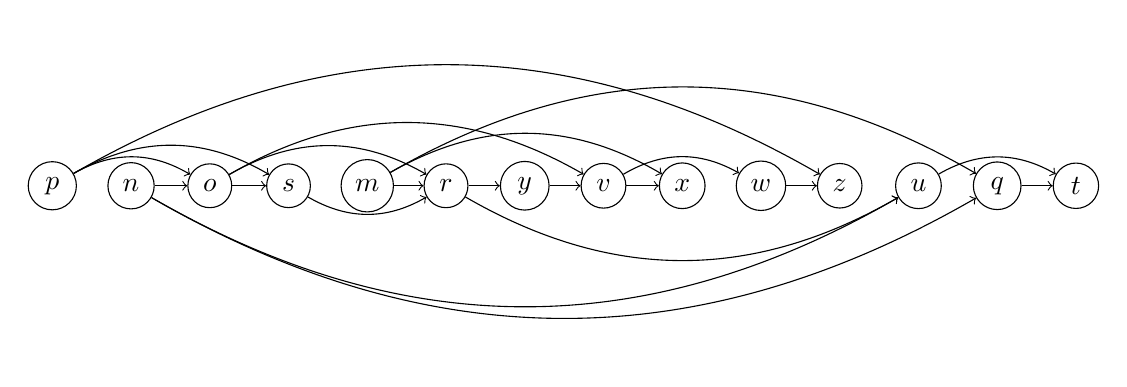
\begin{tikzpicture}
    \tikzset{vertex/.style = {shape=circle,draw,minimum size=1em}}
    \tikzset{edge/.style = {->,> = latex'}}
    \node[vertex] (p) at (0,0) {$p$};
    \node[vertex] (n) at (1,0) {$n$};
    \node[vertex] (o) at (2,0) {$o$};
    \node[vertex] (s) at (3,0) {$s$};
    \node[vertex] (m) at (4,0) {$m$};
    \node[vertex] (r) at (5,0) {$r$};
    \node[vertex] (y) at (6,0) {$y$};
    \node[vertex] (v) at (7,0) {$v$};
    \node[vertex] (x) at (8,0) {$x$};
    \node[vertex] (w) at (9,0) {$w$};
    \node[vertex] (z) at (10,0) {$z$};
    \node[vertex] (u) at (11,0) {$u$};
    \node[vertex] (q) at (12,0) {$q$};
    \node[vertex] (t) at (13,0) {$t$};
    \draw[->, bend left] (p) to (o);
    \draw[->, bend left] (p) to (s);
    \draw[->, bend left] (p) to (z);
    \draw[->] (n) to (o);
    \draw[->, bend right] (n) to (q);
    \draw[->, bend right] (n) to (u);
    \draw[->, bend left] (o) to (r);
    \draw[->] (o) to (s);
    \draw[->, bend left] (o) to (v);
    \draw[->, bend right] (s) to (r);
    \draw[->, bend left] (m) to (q);
    \draw[->] (m) to (r);
    \draw[->, bend left] (m) to (x);
    \draw[->, bend right] (r) to (u);
    \draw[->] (r) to (y);
    \draw[->] (y) to (v);
    \draw[->, bend left] (v) to (w);
    \draw[->] (v) to (x);
    \draw[->] (w) to (z);
    \draw[->, bend left] (u) to (t);
    \draw[->] (q) to (t);
\end{tikzpicture}

\subsection*{22.4-2}

We can perform topological sort on $G$
and utilize dynamic programming to count simple path in linear time.

Denote $c[u]$ as the number of simple paths from $u$ to $t$ in $G$.
We have the following recursive solution:

\begin{equation*}
    c[u] = 
    \begin{cases}
        1 & \text{if $u = t$,} \\
        0 & \text{if $u.f < t.f$,} \\
        \sum\limits_{(u,v) \in E} c[v] & \text{if $u.f > t.f$.}
    \end{cases}
\end{equation*}

The following bottom-up algorithm runs in $O(V + E)$:

\begin{minted}[xleftmargin=20pt,linenos]{cpp}
// graph must be DAG
// s and t must be in the graph
int CountSimplePaths(Graph& graph, int s, int t)
{
    int u;
    std::vector<int> dp_count(graph.size, 0);
    std::list<int> topo_sort = TopologicalSort(graph);
    // find t
    std::list<int>::reverse_iterator rit = topo_sort.rbegin();
    while (rit != topo_sort.rend())
    {
        if (*rit == s)
        {
            return 0;
        }
        else if (*rit == t)
        {
            ++rit;
            break;
        }
        ++rit;
    }
    // perform dp
    dp_count[t] = 1;
    while (rit != topo_sort.rend())
    {
        u = *rit;
        for (int v : graph.adj[u])
        {
            dp_count[u] += dp_count[v];
        }
        if (u == s)
            break;
        ++rit;
    }
    return dp_count[s];
}
\end{minted}

\subsection*{22.4-3}

A forest contains multiple free trees (components).
By Theorem B.2, $|E| = |V| - 1$ in a free tree.
Hence, we can perform DFS on the graph.
For each component,
if the number of edges is more than the number of vertices,
we can determine the graph contains a cycle.
Hence, we can bound the running time in $O(|V| + |V|) = O(|V|)$.

\begin{minted}[xleftmargin=20pt,linenos]{cpp}
bool DFSVisit(Graph& graph, int u_idx, int& time)
{
    Vertex& u = graph.vertices[u_idx];
    ++time;
    u.discovery_time = time;
    u.color = Color::kGray;
    for (int v_idx : graph.adj[u_idx])
    {
        Vertex& v = graph.vertices[v_idx];
        if (u.prev != v_idx)
        {
            if (v.color == Color::kWhite)
            {
                v.prev = u_idx;
                DFSVisit(graph, v_idx, time);
            }
            else if (v.color == Color::kGray)
            {
                return false;
            }
        }
    }
    u.color = Color::kBlack;
    ++time;
    u.finishing_time = time;
    return true;
}

bool IsAcyclic(Graph& graph)
{
    int time, u_idx;
    for (Vertex& u : graph.vertices)
    {
        u.color = Color::kWhite;
        u.prev = -1;
    }
    time = 0;
    for (u_idx = 0; u_idx < graph.size; ++u_idx)
    {
        if (graph.vertices[u_idx].color == Color::kWhite)
        {
            if (DFSVisit(graph, u_idx, time) == false)
            {
                return false;
            }
        }
    }
    return true;
}
\end{minted}

\subsection*{22.4-4}

The claim is incorrect.
Observed ``bad'' edges produced by topological sort 
are exactly back edges classified durning DFS. 
However, DFS might not minimized back edges.
Consider the following graph:

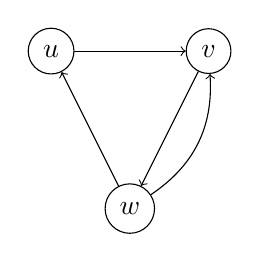
\begin{tikzpicture}
    \tikzset{vertex/.style = {shape=circle,draw,minimum size=1em}}
    \tikzset{edge/.style = {->,> = latex'}}
    \node[vertex] (u) at (0,2) {$u$};
    \node[vertex] (v) at (2,2) {$v$};
    \node[vertex] (w) at (1,0) {$w$};
    \draw[->] (u) to (v);
    \draw[->] (w) to (u);
    \draw[->] (v) to (w);
    \draw[->, bend right] (w) to (v);
\end{tikzpicture}

Let $u$ be our source edge of DFS.
Then we have the following DFS result and topological sort result
which only has two ``bad'' edges: $(w,u)$ and $(w,v)$.

\begin{tabular}{c|c|c}
    vetex & d & f \\
    \hline
    u & 1 & 6 \\
    v & 2 & 5 \\
    w & 3 & 4 \\
\end{tabular}

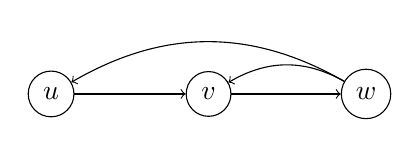
\begin{tikzpicture}
    \tikzset{vertex/.style = {shape=circle,draw,minimum size=1em}}
    \tikzset{edge/.style = {->,> = latex'}}
    \node[vertex] (u) at (0,0) {$u$};
    \node[vertex] (v) at (2,0) {$v$};
    \node[vertex] (w) at (4,0) {$w$};
    \draw[->] (u) to (v);
    \draw[->, bend right] (w) to (u);
    \draw[->] (v) to (w);
    \draw[->, bend right] (w) to (v);
\end{tikzpicture}

However, if we let $w$ be out source edge of DFS and 
let $u$ be in front of $v$ in the adjacency list of $w$,
we have the following DFS result and topological sort result
which has only one ``bad'' edge: $(v, w)$.

\begin{tabular}{c|c|c}
    vetex & d & f \\
    \hline
    u & 2 & 5 \\
    v & 3 & 4 \\
    w & 1 & 6 \\
\end{tabular}

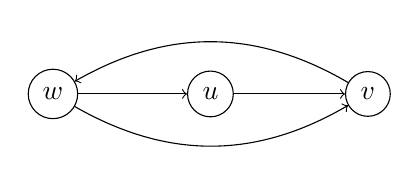
\begin{tikzpicture}
    \tikzset{vertex/.style = {shape=circle,draw,minimum size=1em}}
    \tikzset{edge/.style = {->,> = latex'}}
    \node[vertex] (w) at (0,0) {$w$};
    \node[vertex] (u) at (2,0) {$u$};
    \node[vertex] (v) at (4,0) {$v$};
    \draw[->] (u) to (v);
    \draw[->] (w) to (u);
    \draw[->, bend right] (v) to (w);
    \draw[->, bend right] (w) to (v);
\end{tikzpicture}

\subsection*{22.4-5}

\begin{minted}[xleftmargin=20pt,linenos]{cpp}
std::list<int> TopologicalSort(Graph& graph)
{
    int u;
    std::list<int> topo_sort;
    std::vector<int> in_degree_counter(graph.size, 0);
    std::queue<int> zero_in_degree;
    // compute in-degree
    for (AdjList& adj_list : graph.adj)
    {
        for (int v : adj_list)
        {
            ++in_degree_counter[v];
        }
    }
    // init queue contains vertices with zero in-degree
    for (u = 0; u < graph.size; ++u)
    {
        if (in_degree_counter[u] == 0)
        {
            zero_in_degree.push(u);
        }
    }
    // perform topological sort
    while (zero_in_degree.empty() == false)
    {
        u = zero_in_degree.front();
        zero_in_degree.pop();
        topo_sort.push_back(u);
        for (int v : graph.adj[u])
        {
            --in_degree_counter[v];
            if (in_degree_counter[v] == 0)
            {
                zero_in_degree.push(v);
            }
        }
    }
    return topo_sort;
}
\end{minted}

If the graph has cycles, the array (std::vector) ``in\_degree\_counter'' 
contains non-zero values at the end of the procedure,
so there exist some vertices not contained in
the result of topological sort.

\section*{22.5}

\subsection*{22.5-1}

The number of strongly connected components of a graph will 
stay same or decrease if a new edge is added.

\subsection*{22.5-2}

By Exercise 22.3-2, the result of $\proc{DFS}(G)$ (the first DFS) is the following:

\begin{tabular}{c|c|c}
    vetex & d & f \\
    \hline
    q & 1 & 16 \\
    s & 2 & 7 \\
    v & 3 & 6 \\
    w & 4 & 5 \\
    t & 8 & 15 \\
    x & 9 & 12 \\
    z & 10 & 11 \\
    y & 13 & 14 \\
    r & 17 & 20 \\
    u & 18 & 19 \\
\end{tabular}

Hence $\proc{DFS}(G^T)$ (the second DFS), in the main loop of DFS, 
consider the vetices in the following order:
r u q t y x z s v w.

Therefore, the strongly connected components of the graph is the following:

\begin{description}
    \item r
    \item u
    \item q y t
    \item x z
    \item s w v
\end{description}

\subsection*{22.5-3}

The claim is incorrect.

Construct the sequence $A = \langle a_1, a_2, \cdots, a_{|V|} \rangle$
where $a_i \in V$ for $i \in [1, |V|]$.
WLOG, let $a_i.f$ to be strictly increase for $i \in [1, |V|]$.
Let $C$ be arbitrary strongly connected component.
Let $B = \langle b_1, b_2, \cdots, b_{|C|} \rangle$ be the subsequence of $A$
such that elements in $B$ are vertex of $C$.
Note that $f(C) = \mathop{\func{max}}\limits_{u \in C} \{ u.f \}$.
This says $f(C) = b_{|C|}.f$.
In the main loop of the second DFS,
the procedure consider the vetices in the order of $A$.
This says, in the case of $|C| > 1$,
the procedure will consider $b_1$ before consider $b_{|C|}$,
unlike the process in $\proc{Strongly-Connected-Components}$.
However, we have $b_1.f = \mathop{\func{min}}\limits_{u \in C} \{ u.f \}$.
Let $C'$ be a strongly connected component that is distinct from $C$.
Hence, by lemma 22.14, there might be a edge $(b_1, v)$ where $v \in C'$
and $b_1.f < v.f \leq f(C') < f(C)$ (especially $b_1.f < f(C')$),
which means depth-first forest produced by the second DFS
might not output strongly connected components correctly.

Consider the following counterexample:

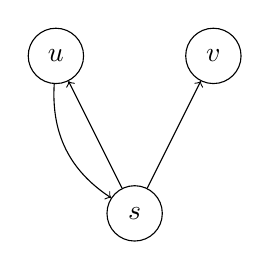
\begin{tikzpicture}
    \tikzset{vertex/.style = {shape=circle,draw,minimum size=2em}}
    \tikzset{edge/.style = {->,> = latex'}}
    \node[vertex] (s) at (1,0) {$s$};
    \node[vertex] (u) at (0,2) {$u$};
    \node[vertex] (v) at (2,2) {$v$};
    \draw[->] (s) to (u);
    \draw[->, bend right] (u) to (s);
    \draw[->] (s) to (v);
\end{tikzpicture}

Let $s$ be the source vertex in the first DFS, 
and let $u$ be in front of $v$ in the adjacency list of $s$.
The result of the first DFS is the following:

\begin{tabular}{c|c|c}
    vetex & d & f \\
    \hline
    s & 1 & 6 \\
    u & 2 & 3 \\
    v & 4 & 5 \\
\end{tabular}

Then the second DFS, in the main loop, 
will consider the vetices in the following order:
u v s.
Hence the second DFS will produce the following depth-first forest:

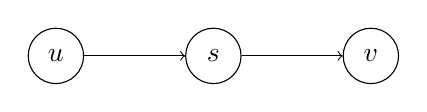
\begin{tikzpicture}
    \tikzset{vertex/.style = {shape=circle,draw,minimum size=2em}}
    \tikzset{edge/.style = {->,> = latex'}}
    \node[vertex] (s) at (2,0) {$s$};
    \node[vertex] (u) at (0,0) {$u$};
    \node[vertex] (v) at (4,0) {$v$};
    \draw[->] (u) to (s);
    \draw[->] (s) to (v);
\end{tikzpicture}

The depth-first forest implies u-s-v are in a single strongly connected component,
which is incorrect.

\subsection*{22.5-4}

\begin{proof}
    Let $G^{SCC} = (V^{SCC}, E^{SCC})$,
    Observed that $G$ and $G^T$ have exactly the same strongly connected components
    (page 616),
    we have $(G^T)^{SCC} = (V^{SCC}, (E^T)^{SCC})$.
    To show $G^{SCC} = ((G^T)^{SCC})^T$,
    we claim $E^{SCC} = ((E^T)^{SCC})^T$.

    ($\subseteq$)
    Suppose that $(u,v) \in E^{SCC}$.
    Then $u,v \in V^{SCC}$
    and $(u,v) \in E$ where $u$ and $v$ are in distinct components.
    By definition of $E^T$, $(v,u) \in E^T$.
    Since $u$ and $v$ are in distinct components
    and $u,v \in V^{SCC}$,
    we have $(v,u) \in (E^T)^{SCC}$.
    Hence $(u,v) \in ((E^T)^{SCC})^T$.

    ($\supseteq$)
    Similar to the proof of ($\subseteq$).
\end{proof}

\subsection*{22.5-5}

\begin{minted}[xleftmargin=20pt,linenos]{cpp}
void DFSVisitComputeComponentGraph(Graph& graph, int u_idx, 
    std::list<int>& adj_list)
{
    Vertex& u = graph.vertices[u_idx];
    for (int v_idx : graph.adj[u_idx])
    {
        Vertex& v = graph.vertices[v_idx];
        if (v.component < 0)
        {
            v.component = u.component;
            DFSVisitComputeComponentGraph(graph, v_idx, adj_list);
        }
        else if (v.component != u.component)
        {
            adj_list.push_back(v.component);
        }
    }
}

std::list< std::list<int> > DFSComputeComponentGraphAdjList(Graph& graph, 
    const std::list<int>& order)
{
    int curr_component, v_idx;
    std::list< std::list<int> > adj_lists;
    for (Vertex& u : graph.vertices)
    {
        u.component = INT_MIN;
    }
    curr_component = 0;// index of component graph start from 0
    for (int u_idx : order)
    {
        Vertex& u = graph.vertices[u_idx];
        if (u.component < 0)
        {
            // DFS find edges (in adj_list) connected with curr_component
            u.component = curr_component;
            adj_lists.emplace_back(std::list<int>());
            DFSVisitComputeComponentGraph(graph, u_idx, adj_lists.back());
            ++curr_component;
        }
    }
    return adj_lists;
}

Graph ComponentGraphAdjLists(Graph& graph)
{
    int i;
    std::list<int> topo_sort = TopologicalSort(graph);
    Graph tranpose = Transpose(graph);
    std::list< std::list<int> > tranpose_component_graph_adj_lists = 
        DFSComputeComponentGraphAdjList(tranpose, topo_sort);
    // build ComponentGraph
    Graph component_graph(tranpose_component_graph_adj_lists.size());
    std::list< std::list<int> >::iterator adj_lists_it = 
        tranpose_component_graph_adj_lists.begin();
    for (i = 0; i < component_graph.size; ++i)
    {
        // adjacency list might exist repeat elements
        // we delete repeat elements by utilizing counter
        // Note that the adjacency list is for (G^T)^{SCC}
        // By Exercise 22.5-4, we showed that G^{SCC} = ((G^T)^{SCC})^T
        std::vector<bool> counter(i + 1, false);
        for (std::list<int>::iterator it = adj_lists_it->begin();
            it != adj_lists_it->end(); ++it)
        {
            if (counter[*it] == false)
            {
                counter[*it] = true;
                component_graph.adj[*it].push_back(i);
            }
        }
        ++adj_lists_it;
    }
    for (i = 0; i < graph.size; ++i)
    {
        component_graph.vertices_lists_from_original_graph
            [tranpose.vertices[i].component].push_back(i);
    }
    return component_graph;
}
\end{minted}

\subsection*{22.5-6}

Notice that a simple directed cycle constructed by vertices of the component
minimized edges in each component.
We can utilize the procedure in 25.5-5 to get component graph in $O(V + E)$.
Therefore, we have the following algorithm which takes $O(V + E)$ time:

\begin{minted}[xleftmargin=20pt,linenos]{cpp}
Graph CreateGraphExercise22_5_6(Graph& graph)
{
    int component_idx, u;
    Graph component_graph = ComponentGraphAdjLists(graph);
    Graph result_graph(graph.size);
    for (component_idx = 0; component_idx < component_graph.size; ++component_idx)
    {
        // build cycle
        std::list<int>& vertices = 
            component_graph.vertices_lists_from_original_graph[component_idx];
        if (vertices.front() != vertices.back())
        {
            u = vertices.back();
            for (int v : vertices)
            {
                result_graph.adj[u].push_back(v);
                u = v;
            }
        }
        // build edges among components
        u = vertices.front();
        std::list<int>& adj = component_graph.adj[component_idx];
        for (int c : adj)
        {
            int v = component_graph.vertices_lists_from_original_graph[c].front();
            result_graph.adj[u].push_back(v);
        }
    }
    return result_graph;
}
\end{minted}

\subsection*{22.5-7}

Let $G = (V,E)$ and $G^{SCC} = (V^{SCC},E^{SCC})$.
Suppose that $G$ has strongly connected components $C_1,C_2,\cdots,C_k$.
The vertex set $V^{SCC}$ is $\{ s_1, s_2, \cdots, s_k \}$,
and it contains a vertex $s_i$ for each strongly connected component $C_i$ of $G$.

\begin{lemma}
    Let $x \in C_i$ and $y \in C_j$.
    $x \leadsto y \Longleftrightarrow s_i \leadsto s_j$ 
\end{lemma}

\begin{proof}
    ($\Longrightarrow$)
    Suppose that $x \leadsto y$.
    Then $\exists w_1, w_2, \cdots, w_p \in V$ such that
    $(x,w_1), (w_1,w_2), \cdots, (w_p,y) \in E$.
    Suppose that $c_1, c_2, \cdots c_p$ are the indexs of components contain $w_1, w_2, \cdots, w_p$;
    i.e. $w_l \in C_{c_l}$ for all $l \in [1,p]$.
    By definition of $E^{SCC}$,
    we have $(s_i,s_{c_1}),(s_{c_1},s_{c_2}), \cdots, (s_{c_j},s_j) \in E^{SCC}$.
    Thus, $s_i \leadsto s_j$.

    ($\Longleftarrow$)
    Suppose that $s_i \leadsto s_j$.
    Then $\exists w_1, w_2, \cdots, w_p \in V^{SCC}$ such that
    $(s_i,w_1), (w_1,w_2), \cdots, (w_p,s_j) \in E^{SCC}$.
    Suppose that $c_1, c_2, \cdots c_p$ are the indexs of components $w_1, w_2, \cdots, w_p$;
    i.e. $w_l = s_{c_l}$ for all $l \in [1,p]$.
    Pick arbitrary $u_l \in C_{c_l}$ for all $l \in [1,p]$.
    By definition of strongly connected components and $E^{SCC}$,
    we have $x \leadsto u_1 \leadsto u_2 \cdots u_p \leadsto y$.
    Thus, $x \leadsto y$.
\end{proof}

\begin{lemma}
    $G$ is semiconnected if and only if
    $G^{SCC}$ is semiconnected.
\end{lemma}

\begin{proof}
    ($\Longrightarrow$)
    Suppose that $G$ is semiconnected.
    That is $\forall x,y \in V, x \leadsto y \vee y \leadsto x$.
    We prove by induction on the number of strongly connected components of $G$.
    Our inductive hypothesis is 
    $\forall u,v \in \{ s_1, s_2, \cdots, s_k \}, u \leadsto v \vee v \leadsto u$.
    The base case is when $G$ containes no vertex, which is trivial.
    Suppose that 
    $\forall u,v \in \{ s_1, s_2, \cdots, s_k \}, u \leadsto v \vee v \leadsto u$.
    Let $x \in C_t$ where $t \in [1,k]$ and $y \in C_{k+1}$ be arbitrary choices.
    Since $x,y \in V$, we have $x \leadsto y \vee y \leadsto x$.
    If $x \leadsto y$, then, by lemma 4, we have $s_t \leadsto s_{k+1}$.
    Similarily, if $y \leadsto x$, we have $s_{k+1} \leadsto s_t$.
    Since $t \in [1,k]$ is a arbitrary choice, by induction,
    we conclude $G^{SCC}$ is semiconnected.

    ($\Longleftarrow$)
    Suppose that $G^{SCC}$ is semiconnected.
    That is $\forall x,y \in V^{SCC}, x \leadsto y \vee y \leadsto x$.
    We prove by induction on the number of strongly connectly components of $G$.
    Our inductive hypothesis is 
    $\forall u,v \in C_1 \cup C_2 \cdots C_k, u \leadsto v \vee v \leadsto u$.
    The base case is when $G$ containes no vertex, which is trivial.
    Suppose that 
    $\forall u,v \in C_1 \cup C_2 \cdots C_k, u \leadsto v \vee v \leadsto u$.
    Let $x \in C_t$ where $t \in [1,k]$ and $y \in C_{k+1}$ be arbitrary choices.
    Since $s_t,s_{k+1} \in V^{SCC}$, we have 
    $s_t \leadsto s_{k+1} \vee s_{k+1} \leadsto s_t$.
    If $s_t \leadsto s_{k+1}$, then, by lemma 4, we have $x \leadsto y$.
    Similarily, if $s_{k+1} \leadsto s_t$, we have $y \leadsto x$.
    Since $t \in [1,k]$ is a arbitrary choice, by induction,
    we conclude $G$ is semiconnected.
\end{proof}

\begin{lemma}
    $G$ is semiconnected if and only if
    we are able to put all elements of $V$ in a sequence 
    $\langle v_1, v_2, \cdots, v_{|V|} \rangle$ such that 
    $v_1 \leadsto v_2 \cdots v_{|V|-1} \leadsto v_{|V|}$.
\end{lemma}

\begin{proof}
    ($\Longrightarrow$)
    Suppose that $G$ is semiconnected.
    That is $\forall u,v \in V, u \leadsto v \vee v \leadsto u$.
    Let $A = \langle a_1, a_2, \cdots, a_k \rangle$ be a sequence.
    We prove by induction on $k$.
    The base case is $k=0$, which is trivial.
    Suppose that
    $a_1 \leadsto a_2 \cdots a_{k-1} \leadsto a_k$.
    Pick arbitrary element $u \in V$ and $u \notin A$.
    If $\exists i \in [1,k)$ such that 
    $a_i \leadsto u \leadsto a_{i+1}$,
    then we insert $u$ between $a_i$ and $a_{i+1}$;
    otherwise, insert $u$ before $a_1$ or after $a_k$ appropriately.
    Re-assigning index of $A$,
    we get $A = \langle a_1, a_2, \cdots, a_k, a_{k+1} \rangle$
    where $a_1 \leadsto a_2 \cdots a_k \leadsto a_{k+1}$.

    ($\Longleftarrow$)
    Immediately.
\end{proof}

\begin{lemma}
    Let $G$ be arbitrary DAG.
    If we are able to put all elements of $V$ in a sequence 
    $\langle v_1, v_2, \cdots, v_{|V|} \rangle$ such that 
    $v_1 \leadsto v_2 \cdots v_{|V|-1} \leadsto v_{|V|}$,
    then $\{ (v_1,v_2), (v_2,v_3), \cdots, (v_{|V|-1}, v_{|V|}) \} \subseteq E$ and
    the result of topological sort order of $G$ is
    $v_1, v_2, \cdots, v_{|V|}$.
\end{lemma}

\begin{proof}
    Suppose that $v_1 \leadsto v_2 \cdots v_{|V|-1} \leadsto v_{|V|}$.
    If $|V|=1$, the lemma is trivial correct.
    Let integer $i \in [1,|V|)$.
    Assume $(v_i, v_{i+1}) \notin E$, for the purpose of contradiction.
    Then $\exists j \neq i, i+1$ such that 
    $v_i \leadsto v_j \leadsto v_{i+1}$.
    If $|V|=2$, we obviously have a contradiction.
    If $j < i$, we have 
    $v_i \leadsto v_j$ and $v_j \leadsto v_i$.
    If $j > i+1$, we have 
    $v_j \leadsto v_{i+1}$ and $v_{i+1} \leadsto v_j$.
    Contradict to $G$ is a DAG.
    
    In order to get other order of $\langle v_1, v_2, \cdots, v_{|V|} \rangle$.
    we must swap some elements in the sequence, and no linear ordering is possible,
    which contradicts to the definition of topological sort.
\end{proof}

\begin{theorem}{(Correctness)}
    Suppose that the result of topological sort order of $G^{SCC}$ is
    $v_1, v_2, \cdots, v_{|V^{SCC}|}$.
    $G$ is semiconnected if and only if 
    $\{ (v_1,v_2), (v_2,v_3), \cdots, (v_{|V^{SCC}|-1}, v_{|V^{SCC}|}) \} \subseteq E^{SCC}$
\end{theorem}

\begin{proof}
    $G$ is semiconnected
    $\overset{\text{lemma 5}}{\Longleftrightarrow}$
    $G^{SCC}$ is semiconnected
    $\overset{\text{lemma 6}}{\Longleftrightarrow}$\\
    $\exists \langle v_1, v_2, \cdots, v_{|V^{SCC}|} \rangle$ where $v \in V^{SCC}$ such that 
    $v_1 \leadsto v_2 \cdots v_{|V^{SCC}|-1} \leadsto v_{|V^{SCC}|}$

    ($\Longrightarrow$)
    Suppose that $v_1 \leadsto v_2 \cdots v_{|V^{SCC}|-1} \leadsto v_{|V^{SCC}|}$.
    Since $G^{SCC}$ is a DAG,
    by lemma 7, we have $\{ (v_1,v_2), (v_2,v_3), \cdots, (v_{|V|-1}, v_{|V|}) \} \subseteq E$.

    ($\Longleftarrow$)
    Suppose that $\{ (v_1,v_2), (v_2,v_3), \cdots, (v_{|V^{SCC}|-1}, v_{|V^{SCC}|}) \} \subseteq E^{SCC}$.
    Then, obviously, we have $v_1 \leadsto v_2 \cdots v_{|V^{SCC}|-1} \leadsto v_{|V^{SCC}|}$.
\end{proof}

Therefore, we have the following $O(V + E)$ algorithm:

\begin{minted}[xleftmargin=20pt,linenos]{cpp}
bool Semiconnected(Graph& graph)
{
    int u;
    Graph component_graph = ComponentGraphAdjLists(graph);
    std::list<int> topo_sort = TopologicalSort(component_graph);
    std::list<int>::iterator it = topo_sort.begin();
    std::list<int>::iterator end = topo_sort.end();
    u = *it;
    ++it;
    while (it != end)
    {
        if (std::find(component_graph.adj[u].begin(), component_graph.adj[u].end(), 
            *it) == component_graph.adj[u].end())
            return false;
        u = *it;
    }
    return true;
}
\end{minted}

\section*{Chapter 22 Problems}

\subsection*{22-1}

\subsubsection*{(a)}

\begin{claim}
    There are no back edges in a BFS of an undirected graph.
\end{claim}

\begin{proof}
    Let $G = (V,E)$ be an undirected graph.
    Suppose that $(u,v) \in E$ is a back edge, for the purpose of contradiction.
    Then $v$ is an ancestor of $u$ in a breadth-first tree.
    If $u.\pi = v$, then $(v,u)$ should be classified as a tree edge
    before $(u,v)$ is classifed as a back edge.
    Now, consider the case of $u.\pi \neq v$.
    That is $(v,w_1), (w_1,w_2), \cdots, (w_{k-1},w_k), (w_k, u) \in E_\pi$
    for some $k \in \NN$.
    We have $u.\pi = w_k$.
    However, since $(u,v) \in E$, we have $(v,u) \in E$,
    and $(v,u)$ should be searched before $(w_k, u)$ is searched,
    so $u.\pi$ should be $v$, and $(v,u)$ should be classified as a tree edge.
    Contradiction.
\end{proof}

\begin{claim}
    There are no forward edges in a BFS of an undirected graph.
\end{claim}

\begin{proof}
    Let $G = (V,E)$ be an undirected graph.
    Suppose that $(u,v) \in E$ is a forward edge, for the purpose of contradiction.
    Then $v$ is an descendant of $u$ in a breadth-first tree.
    If $v.\pi = u$, then $(u,v)$ should be classified as a tree edge.
    Now, consider the case of $v.\pi \neq u$.
    That is $(u,w_1), (w_1,w_2), \cdots, (w_{k-1},w_k), (w_k, v) \in E_\pi$
    for some $k \in \NN$.
    We have $v.\pi = w_k$.
    However, since $(u,v) \in E$,
    $(u,v)$ should be searched before $(w_k, v)$ is searched,
    so $v.\pi$ should be $u$, and $(u,v)$ should be classified as a tree edge.
    Contradiction.
\end{proof}

\begin{claim}
    In a BFS of an undirected graph,
    for each tree edge $(u,v)$, we have $v.d=u.d+1$.
\end{claim}

\begin{proof}
    Let $G = (V,E)$ be an undirected graph.
    Suppose that $(u,v) \in E$ is a tree edge.
    By definition, $v$ was first discovered by exploring edge $(u,v)$.
    Hence line 15 of $\proc{BFS}$ must be performed,
    which is setting $v.d = u.d + 1$.
\end{proof}

\begin{claim}
    In a BFS of an undirected graph,
    for each cross edge $(u,v)$, we have $v.d=u.d$ or $v.d=u.d+1$.
\end{claim}

\begin{proof}
    Let $G = (V,E)$ be an undirected graph.
    Suppose that $(u,v) \in E$ is a cross edge.
    Suppose that $v.d \neq u.d$ and $v.d \neq u.d+1$,
    for the purpose of contradiction.
    That is $u.d > v.d$ or $v.d > u.d +1$.
    $u.d > v.d$ is impossible since $u$ is discovered before $v$.
    Note that $u$ and $v$ must be in a same breath-first tree
    since $(u,v) \in E$ and $G$ is a undirected graph.
    Since $v.d > u.d + 1$, we have $(w,v) \in E$ 
    for some $w \in V \setminus \{ u, v \}$
    where $w.d = v.d - 1$ and $v.\pi = w$.
    Then $w.d > u.d$.
    By lemma 22.3, $u$ is dequeued before $w$.
    Then, when $u$ is dequeued,
    $w.color$ is WHITE or GRAY,
    so $v.color$ is WHITE.
    However, since $(u,v) \in E$ and $v.color$ is WHITE,
    $v.\pi$ will become $u$,
    which means $(u,v)$ is a tree edge.
    Contradiction.
\end{proof}

\subsubsection*{(b)}

\begin{claim}
    There are no forward edges in a BFS of an directed graph.
\end{claim}

\begin{proof}
    Same as the proof of claim 10.
\end{proof}

\begin{claim}
    In a BFS of an directed graph,
    for each tree edge $(u,v)$, we have $v.d=u.d+1$.
\end{claim}

\begin{proof}
    Same as the proof of claim 11.
\end{proof}

\begin{claim}
    In a BFS of an directed graph,
    for each cross edge $(u,v)$, we have $v.d \leq u.d+1$.
\end{claim}

\begin{proof}
    Let $G = (V,E)$ be an directed graph.
    Suppose that $(u,v) \in E$ is a cross edge.
    Then $v.color$ must be GRAY or BLACK when $(u,v)$ is explored.
    Suppose that $v.d > u.d+1$,
    for the purpose of contradiction.
    Then, by lemma 22.3, 
    when $u$ is dequeued, $v$ has not been enqueued yet.
    This says $v.color$ is WHITE at the time that $u$ is dequeued
    and at the time that $(u,v)$ is explored.
    Contradiction.

    Actually, $v.d \leq u.d+1$ must be true for all kind of edge $(u,v)$
    since ``when $u$ is dequeued, $v$ has not been enqueued''
    is contradicting to $(u,v) \in E$ directly.
\end{proof}

\begin{claim}
    In a BFS of an directed graph,
    for each back edge $(u,v)$, we have $0 \leq v.d \leq u.d$.
\end{claim}

\begin{proof}
    Let $G = (V,E)$ be an directed graph.
    Suppose that $(u,v) \in E$ is a back edge.
    Then $v$ is an ancestor of $u$.
    We have $0 \leq v.d \leq u.d$ immediately.
\end{proof}

\subsection*{22-2}

We assume $G = (V,E)$ is a simple, connected, undirected graph
in this problem.

\subsubsection*{(a)}

\begin{claim}
    Let $G = (V,E)$ be a connected, undirected graph.
    Let $s$ be the root of $G_\pi$.
    $s$ is an articulation point of $G$ if and only if
    $s$ has at least two children in $G_\pi$.
\end{claim}

\begin{proof}
    ($\Longrightarrow$)
    Suppose that $s \in V$ is the root of $G_\pi$ 
    and is an articulation point of $G$.
    Let $G' = (V',E')$ be the graph if we remove $s$
    (i.e. $V' = V \setminus \{ s \}$ 
    and $E'$ does not contain a edge connected $s$).
    Since $s$ is an articulation point of $G$,
    there exists two non-empty, disjoint set $W, U \subseteq V'$
    (i.e. $W, U \neq \emptyset$ and $W \cap U = \emptyset$)
    such that for every $w \in W$ and $u \in U$,
    $w \not\leadsto u$ and $u \not\leadsto w$
    in $G'$.

    Suppose that $v \in V$ is the only one child $s$ has in $G.\pi$,
    for the purpose of contradiction.
    Let $E.\pi' = E.\pi \setminus \{ (s,v) \}$
    and $G.\pi' = (V',E.\pi')$.
    Then $E.\pi' \subseteq E'$
    since $(s,v)$ is the only edge in $E.\pi$ that connects $s$.
    Since $G$ is a connected, undirected graph,
    by Theorem 22.10,
    $G.\pi$ must be connected also.
    WLOG, assume $v \in W$ and $v \notin U$.
    Let $u$ be any vertex in $U$.
    Then $u$ is a descendant of $v$ in $G.\pi$
    since $G.\pi$ is a tree 
    where $s$ is the root and $v$ is the only child of $s$.
    Then there exist a path $v \leadsto u$ in $G.\pi$
    that does not visit $s$.
    Thus, such path is in $G.\pi'$ also.
    Since $E.\pi' \subseteq E'$,
    this path is in $G'$.
    Contradiction.

    ($\Longleftarrow$)
    Suppose that $s$ be the root of $G_\pi$.
    Let $C \subseteq V$ contains children of $s$.
    Let $u,w \in C$ where $u \neq w$.
    Let $U$ contains vertices in the subtree rooted at $u$.
    Let $W$ contains vertices in the subtree rooted at $w$.
    We claim for all $x \in U$ and $y \in W$,
    $x \leadsto y$ in $G$ must visit $s$.
    Then removing $s$ will lead to disconnection of $U$ and $W$.

    Suppose that there exist a path $x \leadsto y$ in $G$
    that does not visit $s$, for the purpose of contradiction.
    Then $(a,b) \in E$ for some $a \in U$ and $b \in W$.
    WLOG, assume $u$ is explored before $w$ in DFS.
    By Theorem 22.9 (White-path theorem),
    $w$ is a descendant of $u$ in $G.\pi$,
    which contradicts to $u,w$ is children of $s$.
\end{proof}

\subsubsection*{(b)}

\begin{proof}
    Let $v$ be a nonroot vertex of $G_\pi$.
    
    ($\Longrightarrow$)
    Suppose that $v$ is an articulation point of $G$.
    $v$ must have a child; 
    otherwise, removing $v$ will even not lead $G_\pi$ disconnected,
    and $G$ will naturally be disconnected.
    For the purpose of contradiction,
    suppose that for every subtree rooted at a child of $v$,
    there exist a vertex $u$ in this subtree such that 
    there is a back edge from $u$ to a proper ancestor of $v$.
    Then removing $v$ will not disconnect $G$.
    Contradiction.

    ($\Longleftarrow$)
    Suppose that $v$ has a child $s$ such that
    there is no back edge from $s$ or any descendant of $s$
    to a proper ancestor of $v$.
    Let $S$ be the subtree rooted at $s$ 
    ($S$ is a subgraph of $G_\pi$).
    Then there is no back edge from vertices in $S$ 
    to a proper ancestor of $v$.
    By Theorem 22.10,
    every edge from vertices in $S$ to a proper ancestor is a tree edge.
    Then removing $v$ will cause subtree $S$ being disconnected
    from other part of $G$.
\end{proof}

\subsubsection*{(c)}

\begin{minted}[xleftmargin=20pt,linenos]{cpp}
void DFSVisit(Graph& graph, int u_idx, int& time)
{
    Vertex& u = graph.vertices[u_idx];
    ++time;
    u.discovery_time = time;
    u.color = Color::kGray;
    u.low = u.discovery_time;
    for (int v_idx : graph.adj[u_idx])
    {
        Vertex& v = graph.vertices[v_idx];
        if (v.color == Color::kWhite)
        {
            // tree edge
            v.prev = u_idx;
            DFSVisit(graph, v_idx, time);
            u.low = std::min(u.low, v.low);
        }
        else if (v.color == Color::kGray && u.prev != v_idx)
        {
            // back edge
            u.low = std::min(u.low, v.low);
        }
    }
    u.color = Color::kBlack;
    ++time;
    u.finishing_time = time;
}

void DFS(Graph& graph)
{
    int time, u_idx;
    for (Vertex& u : graph.vertices)
    {
        u.color = Color::kWhite;
        u.prev = -1;
    }
    time = 0;
    for (u_idx = 0; u_idx < graph.size; ++u_idx)
    {
        if (graph.vertices[u_idx].color == Color::kWhite)
        {
            DFSVisit(graph, u_idx, time);
        }
    }
}
\end{minted}

\subsubsection*{(d)}

Let $p$ be a nonroot vertex of $G_\pi$.
$\exists (p,v) \in E_\pi$ such that $v.low \geq p.d \Longleftrightarrow
\not\exists (u,w) \in E$ such that $(u,w)$ is a back edge
$\wedge u$ is a descendant of $v \wedge w$ is a proper ancestor of $p
\Longleftrightarrow p$ is an articulation point

\begin{minted}[xleftmargin=20pt,linenos]{cpp}
void DFSVisit(Graph& graph, int u_idx, int& time, std::list<int>& articulations)
{
    bool is_articulation;
    int tree_edges_counter;
    Vertex& u = graph.vertices[u_idx];
    ++time;
    u.discovery_time = time;
    u.color = Color::kGray;
    u.low = u.discovery_time;
    is_articulation = false;
    tree_edges_counter = 0;
    for (int v_idx : graph.adj[u_idx])
    {
        Vertex& v = graph.vertices[v_idx];
        if (v.color == Color::kWhite)
        {
            // tree edge
            ++tree_edges_counter;
            v.prev = u_idx;
            DFSVisit(graph, v_idx, time, articulations);
            u.low = std::min(u.low, v.low);
            if (v.low >= u.discovery_time)
                is_articulation = true;
        }
        else if (v.color == Color::kGray && u.prev != v_idx)
        {
            // back edge
            u.low = std::min(u.low, v.low);
        }
    }
    u.color = Color::kBlack;
    ++time;
    u.finishing_time = time;
    if ((u.discovery_time != 1 && is_articulation) || 
        (u.discovery_time == 1 && tree_edges_counter >= 2))
        articulations.push_back(u_idx);
}

std::list<int> DFS(Graph& graph)
{
    int time, u_idx;
    std::list<int> articulations;
    for (Vertex& u : graph.vertices)
    {
        u.color = Color::kWhite;
        u.prev = -1;
    }
    time = 0;
    for (u_idx = 0; u_idx < graph.size; ++u_idx)
    {
        if (graph.vertices[u_idx].color == Color::kWhite)
        {
            DFSVisit(graph, u_idx, time, articulations);
        }
    }
    return articulations;
}
\end{minted}

\subsubsection*{(e)}

\begin{proof}
    ($\Longrightarrow$)
    Suppose that $(u,v)$ is an bridge,
    and suppose that $(u,v)$ lies on a simple cycle,
    for the purpose of contradiction.
    Then there exists at least two simple path from $u$ to $v$.
    Disconnecting $(u,v)$,
    we still have a path from $u$ to $v$,
    which means $G$ is still connected.
    Contradiction.

    ($\Longleftarrow$)
    We prove by contrapositive.
    Suppose that $(u,v)$ is not an bridge.
    Then removing $(u,v)$ will not disconnect $G$.
    Hence there must exist another path from $u$ to $v$
    that does not visit $(u,v)$,
    so such path and $(u,v)$ form a simple cycle.
\end{proof}

\subsubsection*{(f)}

$v.low = v.d \Longleftrightarrow
\not\exists (u,w) \in E$ such that $(u,w)$ is a back edge $\wedge$
$u$ is a descendant of $v$ $\wedge$ $w.d < v.d$
$\Longleftrightarrow (v.\pi,v)$ lies on a simple cycle
$\Longleftrightarrow (v.\pi,v)$ is a bridge

\begin{minted}[xleftmargin=20pt,linenos]{cpp}
void DFSVisit(Graph& graph, int u_idx, int& time, 
    std::list< std::pair<int, int> >& bridges)
{
    Vertex& u = graph.vertices[u_idx];
    ++time;
    u.discovery_time = time;
    u.color = Color::kGray;
    u.low = u.discovery_time;
    for (int v_idx : graph.adj[u_idx])
    {
        Vertex& v = graph.vertices[v_idx];
        if (v.color == Color::kWhite)
        {
            // tree edge
            v.prev = u_idx;
            DFSVisit(graph, v_idx, time, bridges);
            u.low = std::min(u.low, v.low);
            if (v.low == v.discovery_time)
                bridges.push_back({ u_idx, v_idx });
        }
        else if (v.color == Color::kGray && u.prev != v_idx)
        {
            // back edge
            u.low = std::min(u.low, v.low);
        }
    }
    u.color = Color::kBlack;
    ++time;
    u.finishing_time = time;
}

std::list< std::pair<int, int> > DFS(Graph& graph)
{
    int time, u_idx;
    std::list< std::pair<int, int> > bridges;
    for (Vertex& u : graph.vertices)
    {
        u.color = Color::kWhite;
        u.prev = -1;
    }
    time = 0;
    for (u_idx = 0; u_idx < graph.size; ++u_idx)
    {
        if (graph.vertices[u_idx].color == Color::kWhite)
        {
            DFSVisit(graph, u_idx, time, bridges);
        }
    }
    return bridges;
}
\end{minted}

\subsubsection*{(g)}

\begin{proof}
    Let $E'$ be the set of the nonbridge edges of $G$ (so $E' \subseteq E$).
    We prove that the biconnected components of $G$ partition $E'$
    by defining a relation $\sim$ on $E'$ and showing it is a equivlence class.
    By the definition of biconnected component,
    the collection of biconnected components of $G$
    is exactly $\quot{E'}{\sim}$.

    For all $(u,v), (x,y) \in E'$, we define relation $\sim$ by 
    $(u,v) \sim (x,y) \Longleftrightarrow (u,v)$ and $(x,y)$
    lies on a common simple cycle of $G$.
    
    (\textit{Reflexivity})
    Let $(u,v) \in E'$.
    Then $(u,v)$ is a nonbridge edge.
    By part (e), $(u,v)$ lies on a simple cycle of $G$.
    Clearly, $(u,v)$ and $(u,v)$ on a common simple cycle.
    Hence $(u,v) \sim (u,v)$.

    (\textit{Symmetry})
    Let $(u,v), (x,y) \in E'$.
    Suppose that $(u,v) \sim (x,y)$.
    Then $(u,v)$ and $(x,y)$ lies on a common simple cycle of $G$.
    It is trivial to show that $(x,y) \sim (u,v)$.

    (\textit{Transitivity})
    Let $(u,v), (x,y), (a,b) \in E'$.
    Suppose that $(u,v) \sim (x,y)$ and $(x,y) \sim (a,b)$.
    Then $(u,v)$ and $(x,y)$ lies on a common simple cycle $C_1$,
    and $(x,y)$ and $(a,b)$ lies on a common simple cycle $C_2$.

    Define symbol
    $u \overset{P}{\leadsto} v$
    as the path from $u$ to $v$ ($u,v \notin P$)
    where $P$ is the set contains vertices on the path from $u$ to $v$.

    WLOG (we can swap ``u'' and ``v'' or swap ``x'' and ``y''), 
    let $u \overset{P_1}{\leadsto} x$ 
    and $v \overset{P_2}{\leadsto} y$ be the simple paths
    that formed cycle $C_1$, so we have $P_1 \cap P_2 = \emptyset$.
    WLOG, let $x \overset{P_3}{\leadsto} a$ 
    and $y \overset{P_4}{\leadsto} b$ be the simple paths
    that formed cycle $C_2$, so we have $P_3 \cap P_4 = \emptyset$.
    Our goal is to form a simple cycle contains $(u,v)$ and $(a,b)$
    by forming path $u \overset{A}{\leadsto} a$
    and $v \overset{B}{\leadsto} b$
    or forming path $u \overset{A}{\leadsto} b$
    and $v \overset{B}{\leadsto} a$
    where $A \cap B = \emptyset$
    Note that we can find non-simple paths 
    for $A$ and $B$
    where $A \cap B = \emptyset$ first
    and transform them into simple paths 
    without changing endpoints and 
    violating $A \cap B = \emptyset$.

    \textbf{Case 1.}
    Construct
    $u \overset{P_5}{\leadsto} a
    = u \overset{P_1}{\leadsto} x \overset{P_3}{\leadsto} a$,
    and construct
    $v \overset{P_6}{\leadsto} b
    = v \overset{P_2}{\leadsto} y \overset{P_4}{\leadsto} b$.
    We have $P_5 \cap P_6 = \emptyset$.
    Transforming $P_5$ and $P_6$ into simple path,
    we can construct the simple cycle by using path $P_5$ and $P_6$.

    \textbf{Case 2.}
    $P_5 \cap P_6 \neq \emptyset$.
    Then $u \overset{P_5}{\leadsto} a
    = u \overset{P_{5.1}}{\leadsto} I_1 \overset{P_{5.2}}{\leadsto} a$
    and $v \overset{P_6}{\leadsto} b
    = v \overset{P_{6.1}}{\leadsto} I_2 \overset{P_{6.2}}{\leadsto} b$
    where $I_1,I_2$ are sets of vertices 
    and $P_5 \cap P_6 \subseteq I_1$, $P_5 \cap P_6 \subseteq I_2$,
    so $(P_{5.1} \cup P_{5.2}) \cap (P_{6.1} \cup P_{6.2}) = \emptyset$.
    Let $I_1.f$ be the first vertex in $I_1$ on the path $u \overset{P_5}{\leadsto} a$
    and $I_1.l$ be the last vertex in $I_1$ on the path.
    Let $I_2.f$ be the first vertex in $I_2$ on the path $v \overset{P_6}{\leadsto} b$
    and $I_2.l$ be the last vertex in $I_2$ on the path.
    WLOG, assume $I_1.f, I_1.l \in I_2$ and $I_2.f, I_2.l \in I_1$.
    We claim \textcircled{1} $x \in P_{5.1}$ and $y \in P_{6.2}$,
    \textcircled{2} $x \in P_{5.2}$ and $y \in P_{6.1}$,
    or \textcircled{3} $x \in I_1$ and $y \in I_2$, and
    show it by contradiction.
    
    Suppose that $x \in I_1$ and $y \notin I_2$, for the purpose of contradiction.
    Then $u \overset{P_5}{\leadsto} a = u \overset{P_{5.1}}{\leadsto} I_{1.1} 
    \overset{\emptyset}{\leadsto} x \overset{\emptyset}{\leadsto}
    I_{1.2} \overset{P_{5.2}}{\leadsto} a$ where $I_1 = I_{1.1} \cup \{ x \} \cup I_{1.2}$.
    We have $P_1 = P_{5.1} \cup I_{1.1}$, $P_3 = I_{1.2} \cup P_{5.2}$, 
    and $I_1.f \in I_{1.1}$, $I_1.l \in I_{1.2}$.
    Since $y \notin I_2$, there are two cases: $I_2 \subseteq P_2$ or $I_2 \subseteq P_4$.
    If $I_2 \subseteq P_2$, then 
    $I_1.f \in I_{1.1} \wedge I_1.f \in I_2 \Longrightarrow I_1.f \in I_{1.1} \cap I_2
    \Longrightarrow I_1.f \in P_1 \cap P_2
    \Longrightarrow P_1 \cap P_2 \neq \emptyset$,
    which is a contradiction.
    If $I_2 \subseteq P_4$, then 
    $I_1.l \in I_{1.2} \wedge I_1.l \in I_2 \Longrightarrow I_1.l \in I_{1.2} \cap I_2
    \Longrightarrow I_1.l \in P_3 \cap P_4
    \Longrightarrow P_3 \cap P_4 \neq \emptyset$,
    which is a contradiction.
    We have a contradiction for $x \notin I_1$ and $y \in I_2$ by the similar way,
    so we conclude $x \in I_1 \Longleftrightarrow y \in I_2$.

    Suppose that $x \in P_{5.1}$ and $y \in P_{6.1}$, for the purpose of contradiction.
    Then $I_1 \subseteq P_3$ and $I_2 \subseteq P_4$.
    Since $I_1 \cap I_2 \neq \emptyset$, we have $P_3 \cap P_4 \neq \emptyset$,
    which is a contradiction.
    We have a contradiction for $x \in P_{5.2}$ and $y \in P_{6.2}$ by the similar way,
    so we conclude $x \notin I_1 \Longrightarrow 
    (x \in P_{5.1} \wedge y \in P_{6.2}) \vee (x \in P_{5.2} \wedge y \in P_{6.1})$.

    We have showed there are only three subcases:
    \textcircled{1} $x \in P_{5.1}$ and $y \in P_{6.2}$,
    \textcircled{2} $x \in P_{5.2}$ and $y \in P_{6.1}$,
    or \textcircled{3} $x \in I_1$ and $y \in I_2$.

    \textcircled{1} Suppose that $x \in P_{5.1}$ and $y \in P_{6.2}$.
    WLOG, assume $I = I_1 = I_2$.
    Then there are two subsubcases according to whether or not 
    $P_1 \cap P_{5.2} = \emptyset \wedge P_4 \cap P_{6.1} = \emptyset$.
    If $P_1 \cap P_{5.2} = \emptyset \wedge P_4 \cap P_{6.1} = \emptyset$,
    we consider paths $u \overset{A}{\leadsto} b = u \overset{P_1}{\leadsto} x 
    \overset{\emptyset}{\leadsto} y \overset{P_4}{\leadsto} b$ and 
    $v \overset{B}{\leadsto} a = 
    v \overset{P_{6.1}}{\leadsto} I \overset{P_{5.2}}{\leadsto} a$.
    We claim $A \cap B = \emptyset$ so we have a simple cycle contains $(u,v)$ and $(a,b)$.
    We need to show that $(P_1 \cup \{ x, y \} \cup P_4) \cap (P_{6.1} \cup I \cup P_{5.2}) = \emptyset$.
    Since $P_1 \cap P_2 = \emptyset$, $P_3 \cap P_4 = \emptyset$, 
    and $u \overset{P_1}{\leadsto} x$, $v \overset{P_2}{\leadsto} y$,
    $x \overset{P_3}{\leadsto} a$, $y \overset{P_4}{\leadsto} b$
    are simple paths,
    We just need to show that $(P_1 \cup P_4) \cap (P_{6.1} \cup P_{5.2}) = \emptyset$.
    Since $(P_{5.1} \cup P_{5.2}) \cap (P_{6.1} \cup P_{6.2}) = \emptyset$,
    we have $P_1 \cup P_{6.1} = \emptyset$ and $P_4 \cup P_{5.2} = \emptyset$.
    By the hypothesis of the subsubcase, we have\
    $P_1 \cup P_{5.2} = \emptyset$ and $P_4 \cup P_{6.1} = \emptyset$.
    Thus, we have showed $A \cap B = \emptyset$ in this subsubcase.
    If $P_1 \cap P_{5.2} \neq \emptyset \vee P_4 \cap P_{6.1} \neq \emptyset$,
    and, WLOG, we assume $P_4 \cap P_{6.1} \neq \emptyset$,
    then $\exists s \in P_4 \cap P_{6.1}$.
    Consider paths $u \overset{A}{\leadsto} a = u \overset{P_5}{\leadsto} a$
    and $v \overset{B}{\leadsto} b = 
    v \overset{P_7}{\leadsto} s \overset{P_8}{\leadsto} a$
    where $P_7 \subseteq P_{6.1}$ and $P_8 \subseteq P_4$.
    We claim $A \cap B = \emptyset$ so we have a simple cycle contains $(u,v)$ and $(a,b)$.
    We need to show that $P_5 \cap (P_7 \cup \{ s \} \cup P_8) = \emptyset$.
    Since $(P_{5.1} \cup P_{5.2}) \cap (P_{6.1} \cup P_{6.2}) = \emptyset$
    and $P_7 \cup \{ s \} \cup P_8 \subseteq P_{6.1} \cup P_{6.2}$,
    we have $(P_{5.1} \cup P_{5.2}) \cap (P_7 \cup \{ s \} \cup P_8) = \emptyset$.
    Since $P_2$ is a simple path,
    we have $I \cap (P_7 \cup \{ s \}) = \emptyset$.
    Since $I \subseteq P_3 \wedge P_8 \subseteq P_4 \wedge P_3 \cap P_4 = \emptyset$,
    we have $I \cap P_8 = \emptyset$.
    Hence we have $I \cap (P_7 \cup \{ s \} \cup P_8) = \emptyset$ also,
    and we have showed $A \cap B = \emptyset$ in this subsubcase.
    In subcase \textcircled{2}, we can form a simple cycle contains $(u,v)$ and $(a,b)$
    and prove it in the similar way of \textcircled{1}.

    \textcircled{3} Suppose that $x \in I_1$ and $y \in I_2$.
    Then we have 
    $u \overset{P_5}{\leadsto} a = u \overset{P_{5.1}}{\leadsto} I_{1.1} 
    \overset{\emptyset}{\leadsto} x \overset{\emptyset}{\leadsto}
    I_{1.2} \overset{P_{5.2}}{\leadsto} a$ where $I_1 = I_{1.1} \cup \{ x \} \cup I_{1.2}$
    and
    $v \overset{P_6}{\leadsto} b = v \overset{P_{6.1}}{\leadsto} I_{2.1} 
    \overset{\emptyset}{\leadsto} y \overset{\emptyset}{\leadsto}
    I_{2.2} \overset{P_{6.2}}{\leadsto} b$ where $I_2 = I_{2.1} \cup \{ y \} \cup I_{2.2}$.
    We have $I_{1.1} \subseteq P_1$, $I_{2.1} \subseteq P_2$, 
    $I_{1.2} \subseteq P_3$, and $I_{2.2} \subseteq P_4$.
    Since $P_1 \cap P_2 = \emptyset$ and $P_3 \cap P_4 = \emptyset$,
    we have $I_{1.1} \cap I_{2.1} = \emptyset$ and $I_{1.2} \cap I_{2.2} = \emptyset$.
    Since $I_1 \cap I_2 = \emptyset$ and $x \notin I_2$, $y \notin I_1$,
    we have $I_{1.1} \cap I_{2.2} \neq \emptyset$ or $I_{1.2} \cap I_{2.1} \neq \emptyset$.
    WLOG, assume $I_{1.2} \cap I_{2.1} \neq \emptyset$.
    
    Similar to \textcircled{1},
    and, WLOG, assume $I = I_{1.2} = I_{2.1}$ and $I' = I_{1.1} = I_{2.2}$,
    there are two subsubcases: 
    if $P_1 \cap P_{5.2} = \emptyset \wedge P_4 \cap P_{6.1} = \emptyset$,
    we have two paths $u \overset{A}{\leadsto} b = u \overset{P_1}{\leadsto} x 
    \overset{\emptyset}{\leadsto} y \overset{P_4}{\leadsto} b$ and 
    $v \overset{B}{\leadsto} a = 
    v \overset{P_{6.1}}{\leadsto} I \overset{P_{5.2}}{\leadsto} a$
    and $A \cap B = \emptyset$;
    if $P_1 \cap P_{5.2} \neq \emptyset \vee P_4 \cap P_{6.1} \neq \emptyset$,
    and, WLOG, we assume $P_4 \cap P_{6.1} \neq \emptyset$,
    then $\exists s \in P_4 \cap P_{6.1}$,
    so we have two paths 
    $u \overset{A}{\leadsto} a = u \overset{P_5}{\leadsto} a$
    and $v \overset{B}{\leadsto} b = 
    v \overset{P_7}{\leadsto} s \overset{P_8}{\leadsto} a$
    where $P_7 \subseteq P_{6.1}$ and $P_8 \subseteq P_{6.2} \subseteq P_4$
    ($P_8 \cap I' = \emptyset$ since $s \notin I'$; 
    otherwise $s \in I' \wedge I' \subseteq P_1 \wedge s \in P_{6.1} \wedge P_{6.1} \subseteq P_2
    \Longrightarrow s \in P_1 \cap P_2$, contradiction)
    and $A \cap B = \emptyset$.
    Thus, we have a simple cycle contains $(u,v)$ and $(a,b)$.

    Therefore, $(u,v) \sim (a,b)$.
    We have showed relation $\sim$ is a equivlence class on $E'$.
\end{proof}

\subsubsection*{(h)}

\begin{lemma}
    Let $G = (V,E)$ be a simple, undirected, connected graph
    and $x,y \in V$.
    After DFS, we have
    $(x.d \leq y.d) \Longrightarrow (\exists$ simple path
    $x \overset{A}{\leadsto} y$
    such that $(\forall a \in A, a.d < y.d))$.
\end{lemma}

\begin{proof}
    If $x$ is an ancestor of $y$,
    we can simply connect tree edges between $x$ and $y$,
    and we have $\forall a \in A, x.d < a.d < y.d$.
    If $x$ is not an ancestor of $y$,
    then let $s$ be the vertex where $s$ is the ancestor of $x$ and $y$
    with the grestest possible $s.d$.
    Note that such $s$ must exist since $G$ is a connected graph.
    Construct $x \overset{A}{\leadsto} y = 
    x \overset{B}{\leadsto} s \overset{C}{\leadsto} y$
    where $x \overset{B}{\leadsto} s$ is formed by connecting
    all tree edges from $x$ to $s$
    and $s \overset{C}{\leadsto} y$ is formed by connecting
    all tree edges from $s$ to $y$,
    so $A = B \cup \{ s \} \cup C$, and
    $B$ and $C$ are simple paths.
    Clearly, $\forall a \in A, a.d < \func{max}(x.d, y.d) = y.d$.
    We also have $B \cap C = \emptyset$
    since otherwise $p.d > s.d$ where $p \in B \cap C$,
    which contradicts $s$ is the candidate with the grestest possible $s.d$.
    Thus, $x \overset{A}{\leadsto} y$ is a simple path.
\end{proof}

\begin{lemma}
    Let $G = (V,E)$ be a simple, undirected, connected graph
    and $u,v \in V$ where $u$ is nonroot vertex of $G_\pi$.
    Let $E'$ be the set of the nonbridge edges of $G$ (so $E' \subseteq E$).
    $(u,v)$ is a back edge $\Longrightarrow 
    (u,v) \in E' \wedge (u,v).bcc = (u.\pi,u).bcc$.
\end{lemma}

\begin{proof}
    Consider the cycle formed by the path
    $v \overset{A}{\leadsto} u.\pi 
    \overset{\emptyset}{\leadsto} u 
    \overset{\emptyset}{\leadsto} v$.
    We construct $u \overset{\emptyset}{\leadsto} v$
    by using the back edge $(u,v)$
    and construct $u.\pi \overset{\emptyset}{\leadsto}$
    by using the tree edge $(u.\pi,u)$ simply.
    Since $(u,v)$ is a back edge,
    we have $v.d < u.d$,
    so $v.d \leq u.\pi.d$.
    By lemma 18, $\exists$ simple path
    $v \overset{A}{\leadsto} u.\pi$
    such that $(\forall a \in A, a.d < u.\pi.d)$.
    Hence $(u,v)$ and $(u.\pi,u)$ lies on the common simple cycle,
    which means $(u,v).bcc = (u.\pi,u).bcc$.
\end{proof}

\begin{claim}
    Let $G = (V,E)$ be a simple, undirected, connected graph
    and $u,v \in V$ where $u$ is nonroot vertex of $G_\pi$.
    Let $E'$ be the set of the nonbridge edges of $G$ (so $E' \subseteq E$).
    After DFS, we have
    $v.low < u.d \Longleftrightarrow 
    (u,v) \in E' \wedge (u,v).bcc = (u.\pi,u).bcc$.
\end{claim}

\begin{proof}
    ($\Longrightarrow$)
    Suppose that $v.low < u.d$.
    
    \textbf{Case 1.}
    $(u,v)$ is tree edge.

    Then $u.d = v.d - 1$ and $\exists (z,w) \in E$ such that
    $(z,w)$ is a back edge $\wedge$ $z$ is a descendant of $v$
    $\wedge$ $w.d < u.d$.
    Hence $w.d \leq u.\pi.d$.
    By lemma 18, $\exists$ simple path
    $w.d \overset{A}{\leadsto} u.\pi$
    such that $(\forall a \in A, a.d < u.\pi.d)$.
    Consider the cycle formed by the path
    $w.d \overset{A}{\leadsto} u.\pi 
    \overset{\emptyset}{\leadsto} u 
    \overset{\emptyset}{\leadsto} v
    \overset{B}{\leadsto} z
    \overset{\emptyset}{\leadsto} w$
    where $v \overset{B}{\leadsto} z$
    is formed by connecting all tree edges from $v$ to $z$
    Since $(\forall a \in A, a.d < u.\pi.d)$,
    $(\forall b \in B, b.d > v.d)$, and $u.\pi.d + 1 = u.d = v.d - 1$,
    we conclude $A \cap B = \emptyset$.
    Therefore, it is a simple cycle, and 
    $(u,v)$ and $(u.\pi,u)$ lies on the common simple cycle,
    which means $(u,v).bcc = (u.\pi,u).bcc$.

    \textbf{Case 2.}
    $(u,v)$ is back edge.
    
    Immediately from lemma 19.

    ($\Longleftarrow$)
    We prove by contrapositive.
    Suppose that $v.low \geq u.d$.
    $(u,v)$ cannot be a back edge;
    otherwise, we have $u.d > v.d \geq v.low$,
    which contradicts to our hypothesis.
    Hence $(u,v)$ is a tree edge.
    Then $u.d = v.d - 1$ and $v.low \geq u.d = v.d - 1$.
    Since $v.low \leq v.d$, 
    there are two case: $v.low = v.d$ or $v.low = v.d - 1$.

    \textbf{Case 1.}
    $v.low = v.d$.

    By part (f), we have $(v.\pi,v) = (u,v)$ is a bridge.
    Hence $(u,v) \notin E'$.

    \textbf{Case 2.}
    $v.low = v.d - 1$.

    Then $(v.\pi,v) = (u,v)$ is not a bridge.
    Hence $(u,v) \notin E'$.
    Suppose that $(u,v).bcc = (u.\pi,u).bcc$,
    for the purpose of contradiction.
    Then $(u,v)$ and $(u.\pi,u)$ lies on a common simple cycle.
    We already have $u.\pi \overset{\emptyset}{\leadsto} u 
    \overset{\emptyset}{\leadsto} v$
    formed by tree edges.
    We also need a back edge $(z,w)$ such that
    $z$ is a descendant of $v$ and $w.d \leq u.\pi.d$.
    Then we have $v.low \leq u.\pi.d$,
    which contradicts to $v.low = v.d - 1 = u.d$.
\end{proof}

\begin{minted}[xleftmargin=20pt,linenos]{cpp}
void DFSVisitLabelVertice(Graph& graph, int u_idx, int& time)
{
    Vertex& u = graph.vertices[u_idx];
    ++time;
    u.discovery_time = time;
    u.color = Color::kGray;
    u.low = u.discovery_time;
    for (Edge& e : graph.adj[u_idx])
    {
        Vertex& v = graph.vertices[e.vertex];
        if (v.color == Color::kWhite)
        {
            // tree edge
            v.prev = u_idx;
            DFSVisitLabelVertice(graph, e.vertex, time);
            u.low = std::min(u.low, v.low);
        }
        else if (v.color == Color::kGray && u.prev != e.vertex)
        {
            // back edge
            u.low = std::min(u.low, v.low);
        }
    }
    u.color = Color::kBlack;
    ++time;
    u.finishing_time = time;
}

void DFSVisitLabelEdges(Graph& graph, int u_idx, int last_bcc, int& bcc_counter)
{
    Vertex& u = graph.vertices[u_idx];
    u.color = Color::kGray;
    for (Edge& e : graph.adj[u_idx])
    {
        Vertex& v = graph.vertices[e.vertex];
        if (v.color == Color::kWhite)
        {
            // tree edge
            if (v.low < u.discovery_time)
                e.bcc = last_bcc;
            else if (v.discovery_time == v.low)
                e.bcc = -1;// bridge edge
            else
                e.bcc = ++bcc_counter;
            
            DFSVisitLabelEdges(graph, e.vertex, e.bcc, bcc_counter);
        }
        else if (v.color == Color::kGray && u.prev != e.vertex)
        {
            // back edge
            e.bcc = last_bcc;
        }
    }
    u.color = Color::kBlack;
}

// graph: simple, connected, undirected
void LabelBcc(Graph& graph)
{
    int time, bcc_counter;
    // first DFS: compute prev, discovery_time, finishing_time, 
    //      low attributes for each vertex
    graph.vertices[0].prev = -1;
    for (Vertex& u : graph.vertices)
    {
        u.color = Color::kWhite;
    }
    time = 0;
    DFSVisitLabelVertice(graph, 0, time);
    // second DFS: label bcc attributes for each edge
    for (Vertex& u : graph.vertices)
    {
        u.color = Color::kWhite;
    }
    bcc_counter = 0;
    DFSVisitLabelEdges(graph, 0, 0, bcc_counter);
}
\end{minted}

\subsection*{22-3}

\subsubsection*{(a)}

\begin{lemma}
    If $\func{in-degree}(v) = \func{out-degree}(v)$
    for each vertex $v \in V$,
    then (for all $u \in V$, 
    $\func{in-degree}(u) = \func{out-degree}(u) \geq 1
    \Longrightarrow
    $($\exists$ cycle contains $u$ and 
    $\func{in-degree}(v) = \func{out-degree}(v)$
    for each vertex $v \in V$
    after removing each edges in the cycle)).
\end{lemma}

Note that the path of a cycle contains at least one edge.

\begin{proof}
    Suppose that $\func{in-degree}(v) = \func{out-degree}(v)$
    for each vertex $v \in V$.
    Let $u \in V$ be arbitrary choice.
    Suppose that $\func{in-degree}(u) = \func{out-degree}(u) \geq 1$.
    We inductively construct an cycle 
    $\langle a_1, a_2, \cdots, a_n \rangle$ 
    contains $u$, where $k$ is our induction varible.
    Let $a_1 = u$.
    Assume we remove the edge after we visited it.
    The base case is $k = 2$:
    since $\func{out-degree}(u) \geq 1$,
    $\exists (u,w) \in E$,
    so we remove $(u,w)$ and let $a_2 = w$,
    and we have $\func{in-degree}(a_1) = \func{out-degree}(a_1) + 1$
    and $\func{in-degree}(a_2) = \func{out-degree}(a_2) - 1$.
    Assume $\func{in-degree}(a_k) = \func{out-degree}(a_k) - 1$
    for some $k \geq 2$
    and $\func{in-degree}(a_j) = \func{out-degree}(a_j)$
    for all $j = 2, \cdots, k-1$,
    which is our inductive hypothesis.
    Then $\func{out-degree}(a_k) = \func{in-degree}(a_k) + 1 \geq 1$.
    We have $\exists (a_k,x) \in E$.
    We remove $(a_k,x)$ and let $a_{k+1} = x$,
    which means $\func{in-degree}(a_{k+1})$ and
    $\func{out-degree}(a_k)$ decreased by $1$.
    If $a_k = u$, then we stop our construction and have a cycle
    contains $u$, and we conclude 
    $\func{in-degree}(v) = \func{out-degree}(v)$
    for all $v \in V$ at this time (after construction of the cycle).
    If $a_k \neq u$, 
    then we have $\func{in-degree}(a_k) = \func{out-degree}(a_k)$
    and $\func{in-degree}(a_{k+1}) = \func{out-degree}(a_{k+1}) - 1$,
    so our inductive hypothesis hold for next induction varible.
\end{proof}

\begin{claim}
    $G$ has an Euler tour
    $\Longleftrightarrow$
    $\func{in-degree}(v) = \func{out-degree}(v)$
    for each vertex $v \in V$.
\end{claim}

\begin{proof}
    ($\Longrightarrow$)
    We prove by contrapositive.
    Suppose that there exists $v \in V$ such that
    $\func{in-degree}(v) \neq \func{out-degree}(v)$.
    If $\func{in-degree}(v) > \func{out-degree}(v)$,
    then there will be $\func{in-degree}(v) - \func{out-degree}(v)$
    edges to $v$ cannot be visit
    since the tour need to go into $v$ $\func{in-degree}(v)$ times
    and only go out $v$ $\func{out-degree}(v)$ times 
    then the tour will stuck in $v$.
    Similarily, if $\func{in-degree}(v) < \func{out-degree}(v)$,
    then there will be $\func{out-degree}(v) - \func{int-degree}(v)$
    edges from $v$ cannot be visit.
    Hence $G$ does not have an Euler tour.

    ($\Longleftarrow$)
    Notice the our tour is actually a cycle 
    unless there are only one node in the graph, which is trivial.
    Assume there are at least two nodes in the graph.
    Then we the graph contains at least one cycle.
    Suppose that $\func{in-degree}(v) = \func{out-degree}(v)$
    for each vertex $v \in V$ before we start the construction.
    We inductively construct the set of cycles 
    $S = \{ C : C$ is a cycle$ \}$
    where the induction varible is $|S|$.
    Assume we remove the edges that in the cycles from the graph.
    The inductive hypothesis is
    $\func{in-degree}(v) = \func{out-degree}(v)$
    for all $v \in V$.
    The base case is $|S| = 0$,
    which is before the start of the construction
    By our hypothesis of the problem,
    the inductive hypothesis hold for next step.
    Suppose that the inductive hypothesis is true
    after cycles in $S$ are constructed where $|S| = k$.
    If $\exists u \in V$ such that 
    $\func{in-degree}(u) = \func{out-degree}(u) \geq 1$,
    then by lemma 21, we have a cycle $C$ contains $u$.
    We insert this $C$ into the set $S$ and $|S| = k + 1$.
    Since $\func{in-degree}(v) = \func{out-degree}(v)$
    for each vertex $v \in V$
    after removing each edges in the cycle $C$,
    our inductive hypothesis hold for next step.
    If $\forall u \in V$,
    $\func{in-degree}(u) = \func{out-degree}(u) = 0$,
    then we stop the indcution and all edges are removed (visited).

    Now we reconsider the removed edges, 
    and we have cycles in $S$ contains all edges in the graph.
    In order to form an Euler tour, 
    we just need to merge these cycles to a single cycle,
    which is exactly our Euler tour.
    If $|S|=1$, then the only cycle in $S$ is our Euler tour.
    If $|S| > 1$, then we claim 
    $\exists C, D \in S$ where
    $C = \langle c_1, c_2, \cdots, c_m \rangle$ and
    $D = \langle d_1, d_2, \cdots, d_n \rangle$ 
    such that $c_i = d_j$ 
    for some integers $i \in [1,m]$ and $j \in [1,n]$;
    otherwise, the graph is not strongly connected.
    We merge $C$ and $D$ at the vertex $c_i = d_j$ by forming cycle 
    $\langle c_1, c_2, \cdots, c_i, 
    d_{j+1}, d_{j+2}, \cdots, d_n, d_1, \cdots, d_{j-1},
    c_{i+1}, \cdots, c_m \rangle$.
    Clearly, we can inductively merge all cycles in $S$
    and find an Euler tour.    
\end{proof}

\subsubsection*{(b)}

\begin{minted}[xleftmargin=20pt,linenos]{cpp}
std::list< std::pair<int, int> > EulerTour(Graph& graph)
{
    int u, v, s;

    if (graph.size <= 1)
        return std::list< std::pair<int, int> >();

    std::vector< AdjList > adjs_copy = graph.adj;// make a copy of adjacency list
    std::list< std::pair<int, int> > tour;// result
    std::vector< std::list< std::pair<int, int> >::iterator > 
        tour_its(graph.size, tour.end());// iterators of tours for each insert-availble 
                                         // (in the tour list) vertices
    std::queue<int> todo;// queue of vertices in the tour list already
    
    todo.push(0);

    while (todo.empty() == false)
    {
        u = todo.front();
        s = u;
        todo.pop();
        std::list< std::pair<int, int> >::iterator tour_curr_it = tour_its[u];
            // current iterator of insert postion in the tour list

        while (adjs_copy[u].empty() == false)
        {
            v = adjs_copy[u].front();
            tour_its[u] = tour.insert(tour_curr_it, { u, v });
            adjs_copy[u].pop_front();
            todo.push(u);
            u = v;
        }

        if (s != u)
            return std::list< std::pair<int, int> >();
    }

    return tour;
}
\end{minted}

\subsection*{22-4}

\textbf{Approach 1}
Find the strongly connected components (SCC) of the graph first.
Each pair in a SCC are reachable each other,
so we can treat each SCC as a whole, and take the minimum value in the SCC
as the value of the SCC.
Then the SCC graph is a DAG, 
so we can utilize a simple dynamic programming.
Define $L(u)$ and $R(u)$ on $G^{SCC} = (V^{SCC}, E^{SCC})$ 
with the same definition of $G$.
Denote $c[u]$ as $\func{min} \{ L(w) : w \in R(u) \}$ 
for all $u \in V^{SCC}$.

\begin{equation*}
    c[u] = \func{min}
    \begin{cases}
        L(u) \\
        \mathop{\func{min}}\limits_{(u,v) \in E^{SCC}}(c[v])\\
    \end{cases}
\end{equation*}

\begin{minted}[xleftmargin=20pt,linenos]{cpp}
void TopoSortVisit(Graph<OriginalVertex>& graph, int u, 
    std::list<int>& topo_sort_result)
{
    graph.vertices[u].color = Color::kNonWhite;
    for (int v : graph.adj[u])
    {
        if (graph.vertices[v].color == Color::kWhite)
            TopoSortVisit(graph, v, topo_sort_result);
    }
    topo_sort_result.push_front(u);
}

// component_adj_list is for tranpose graph and might exist repeat elements 
void SCCTranposeVisit(Graph<TranposeVertex>& tranpose, int u, 
    std::list<int>& component_vertices, std::list<int>& component_adj_list, 
    int curr_component)
{
    tranpose.vertices[u].color = Color::kNonWhite;
    tranpose.vertices[u].component = curr_component;
    component_vertices.push_back(u);
    for (int v : tranpose.adj[u])
    {
        if (tranpose.vertices[v].color == Color::kWhite)
            SCCTranposeVisit(tranpose, v, component_vertices, 
                component_adj_list, curr_component);
        else if (tranpose.vertices[v].component != curr_component)
            // default value of component attribute is INT_MIN
            component_adj_list.push_back(tranpose.vertices[v].component);
    }
}

void DpSCCVisit(Graph<SCCVertex>& scc, int u)
{
    scc.vertices[u].color = Color::kNonWhite;
    for (int v : scc.adj[u])
    {
        if (scc.vertices[v].color == Color::kWhite)
        {
            DpSCCVisit(scc, v);
            if (scc.vertices[u].dp_min_scc_value > scc.vertices[v].dp_min_scc_value)
            {
                scc.vertices[u].dp_min_scc_vertex = scc.vertices[v].dp_min_scc_vertex;
                scc.vertices[u].dp_min_scc_value = scc.vertices[v].dp_min_scc_value;
            }
        }
    }
}

void Reachability(Graph<OriginalVertex>& graph)
{
    int u, component_counter;
    std::list<int> topo_sort_result;
    std::list< std::list<int> > component_vertices_collection, 
        tranpose_component_adj_list_collection;
    // topo sort
    graph.WhitenAllVertices();
    for (u = 0; u < graph.size; ++u)
    {
        if (graph.vertices[u].color == Color::kWhite)
            TopoSortVisit(graph, u, topo_sort_result);
    }
    // find tranpose
    Graph<TranposeVertex> tranpose = Tranpose(graph);
    // find strongly connected components
    tranpose.WhitenAllVertices();
    component_counter = 0;
    for (int w : topo_sort_result)
    {
        if (tranpose.vertices[w].color == Color::kWhite)
        {
            component_vertices_collection.emplace_back();
            tranpose_component_adj_list_collection.emplace_back();
            SCCTranposeVisit(tranpose, w, component_vertices_collection.back(), 
                tranpose_component_adj_list_collection.back(), component_counter);
            ++component_counter;
        }
    }
    // make scc graph
    Graph<SCCVertex> scc(component_counter);
    u = 0;
    for (std::list<int>& component_vertices : component_vertices_collection)
    {
        scc.vertices[u].vertices.assign(component_vertices.begin(), 
            component_vertices.end());
        ++u;
    }
    u = 0;
    for (std::list<int>& component_adj_list : tranpose_component_adj_list_collection)
    {
        std::vector<bool> repeat_counter(scc.size, false);
        for (int v : component_adj_list)
        {
            if (repeat_counter[v] == false)
            {
                scc.adj[v].push_back(u);
                repeat_counter[v] = true;
            }
        }
        ++u;
    }
    // init dp_min_scc_vertex and dp_min_scc_value for each scc vertex
    for (SCCVertex& scc_v : scc.vertices)
    {
        scc_v.dp_min_scc_vertex = *(std::min_element(scc_v.vertices.begin(), 
            scc_v.vertices.end(), [&graph](int a, int b) { 
                return graph.vertices[a].value < graph.vertices[b].value; 
            }));
        scc_v.dp_min_scc_value = graph.vertices[scc_v.dp_min_scc_vertex].value;
    }
    // dp find min for each scc
    scc.WhitenAllVertices();
    for (u = 0; u < scc.size; ++u)
    {
        if (scc.vertices[u].color == Color::kWhite)
            DpSCCVisit(scc, u);
    }
    // set min attribute for each original vertex
    for (SCCVertex& scc_v : scc.vertices)
    {
        for (int v : scc_v.vertices)
        {
            graph.vertices[v].min = scc_v.dp_min_scc_vertex;
        }
    }
}
\end{minted}

\textbf{Approach 2}
Perform DFS on $G^T$ by considering vertices 
in the increasing order of $L(u)$ in the out-most loop.
The depth-first forest partition vertices with the same $min$
into the same depth-first forest tree where $min$ is the root
vertex of the tree.

The root has the minimum $L$ value due to the order we consider vertices.
The root of the tree of $G^T$ is reachable in $G$ by each vertex 
in the tree of $G^T$. 
The main idea is $u \leadsto v$ in $G$
$\Longleftrightarrow$
$v \leadsto u$ in $G^T$.
Note that DFS will visit all reachable unvisited vertices.
Hence considering vertices in the increasing order of $L(u)$
makes the algorithm work correctly.

\begin{minted}[xleftmargin=20pt,linenos]{cpp}
void DFSVisit(Graph<TranposeVertex>& tranpose, int u, 
    Graph<OriginalVertex>& graph, int root)
{
    tranpose.vertices[u].color = Color::kNonWhite;
    graph.vertices[u].min = root;
    for (int v : tranpose.adj[u])
    {
        if (tranpose.vertices[v].color == Color::kWhite)
            DFSVisit(tranpose, v, graph, root);
    }
}

void Reachability(Graph<OriginalVertex>& graph)
{
    int u;
    std::vector<int> counting_sort(graph.size);
    // sort vertices in the increasing order of L value in linear time
    for (u = 0; u < graph.size; ++u)
    {
        counting_sort[graph.vertices[u].value] = u;
    }
    // find tranpose
    Graph<TranposeVertex> tranpose = Tranpose(graph);
    // DFS
    tranpose.WhitenAllVertices();
    for (int v : counting_sort)
    {
        if (tranpose.vertices[v].color == Color::kWhite)
            DFSVisit(tranpose, v, graph, v);
    }
}
\end{minted}

\end{document}